% Copyright (c) 2014,2016 Casper Ti. Vect 
\chapter{系统详细设计与实现}
在前章中已将本文的系统设计概要架构说明,在本章中将对数据库的内容信息设计进行详细的说明、数据库ER模型架构、各个模块的类与类之间的关系、每个模块运作的顺序以及模块与模块之间的响应关系,最后则是系统实现的平台展示。

	\section{BTMS数据库设计}

	比特币的交易监督系统应用了六个信息表如图\ref{db}所示,分别为商家信息、产品信息、交易信息、用户信息、职工信息以及商家产品信息,以下将逐一说明:

		\begin{figure}[!htbp]
			\centering
			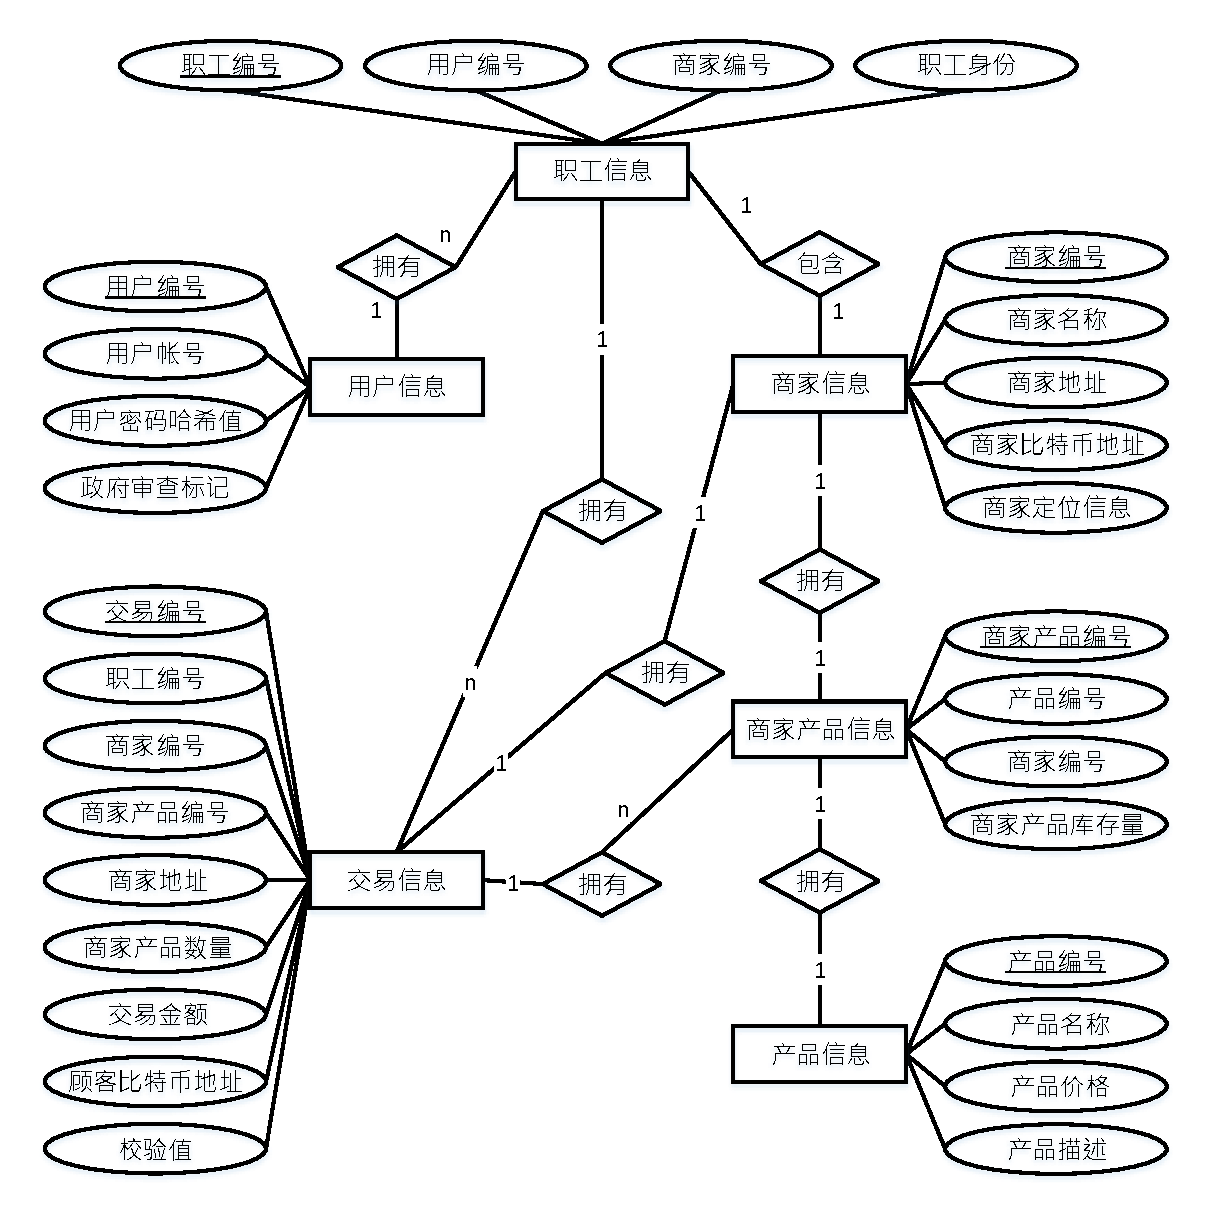
\includegraphics[width = 0.9\textwidth]{er.pdf}
			\caption{BTMS数据库实体关系图}\label{db}
		\end{figure}

		\begin{enumerate}
		\item 商家信息表:存储正在审核中的企业信息或已经过审核的企业信息。表\ref{store}存储的信息包括商家编号、商家名称、商家地址、商家比特币地址以及商家定位信息。


				\begin{table}[!htbp]
				\centering
				\caption{商家信息表}
				\label{store}
				\resizebox{\textwidth}{!}{%
				\begin{tabular}{|c|c|c|c|c|c|}
				\hline
				序号 & 字段名 & 字段说明 & 类型 & 是否为空 & 主外键 \\ \hline
				1 & STORE\_ID & 商家编号 & int & 否 & PK \\ \hline
				2 & STORE\_NAME & 商家名称 & navarchar(20) & 否 &  \\ \hline
				3 & STORE\_ADDRESS & 商家地址 & navarchar(50) & 否 &  \\ \hline
				4 & STORE\_BTCADDRESS & 商家比特币地址 & navarchar(50) & 否 &  \\ \hline
				5 & STORE\_GPS & 商家定位信息 & navarchar(30) & 否 &  \\ \hline
				\end{tabular}%
				}
				\end{table}

		\item 产品信息表:只有授权用户才能登入添加或修改交易产品信息。表\ref{product}产品信息表内容包括产品编号、产品名称、产品价格以及产品描述信息。

				\begin{table}[!htbp]
				\centering
				\caption{产品信息表}
				\label{product}
				
				\begin{tabular}{|c|c|c|c|c|c|}
				\hline
				序号 & 字段名 & 字段说明 & 类型 & 是否为空 & 主外键 \\ \hline
				1 & PRODUCT\_ID & 产品编号 & int & 否 & PK \\ \hline
				2 & PRODUCT\_NAME & 产品名称 & navarchar(10) & 否 &  \\ \hline
				3 & PRODUCT\_PRICE & 产品价格 & float & 否 &  \\ \hline
				4 & PRODUCT\_DESCRIPTION & 产品描述 & navarchar(50) & 是 &  \\ \hline
				\end{tabular}
				\end{table}

		\item 交易信息表:表\ref{tx}记录包括交易编号、职工编号、商家编号、商家产品编号、商家地址、商家产品数量、交易金额、顾客比特币地址和最后确认字段的校验值。

				% \usepackage{graphicx}
				\begin{table}[!htbp]
				\centering
				\caption{交易信息表}
				\label{tx}
				\resizebox{\textwidth}{!}{%
				\begin{tabular}{|c|c|c|c|c|c|}
				\hline
				序号 & 字段名 & 字段说明 & 类型 & 是否为空 & 主外键 \\ \hline
				1 & TX\_ID & 交易编号 & int & 否 & PK \\ \hline
				2 & STAFF\_ID & 职工编号 & int & 否 & FK \\ \hline
				3 & STORE\_ID & 商家编号 & int & 否 & FK \\ \hline
				4 & STOREPRODUCT\_ID & 商家产品编号 & int & 否 & FK \\ \hline
				5 & STORE\_ADDRESS & 商家地址 & navarchar(50) & 否 & FK \\ \hline
				6 & STOREPRODUCT\_QUANTITY & 商家产品数量 & int & 否 &  \\ \hline
				7 & TX\_AMOUNT & 交易金额 & float & 否 &  \\ \hline
				8 & CONSUMER\_BTCADDRESS & 顾客比特币地址 & navarchar(50) & 否 &  \\ \hline
				9 & CHECK & 校验值 & bool & 否 &  \\ \hline
				\end{tabular}%
				}
				\end{table}

		\item 用户信息表:表\ref{user}存储所有用户信息,包括政府、商家及顾客之个人的帐户编号与帐号,而用户密码则以哈希值的方式保存以增加用户安全性,最后则是政府审查值,倘若通过为"1",未通过为"0"。

				\begin{table}[!htbp]
				\centering
				\caption{用户信息表}
				\label{user}
				\resizebox{\textwidth}{!}{%
				\begin{tabular}{|c|c|c|c|c|c|}
				\hline
				序号 & 字段名 & 字段说明 & 类型 & 是否为空 & 主外键 \\ \hline
				1 & USER\_ID & 用户编号 & int & 否 & PK \\ \hline
				2 & USER\_ACCOUNT & 用户帐号 & navarchar(30) & 否 &  \\ \hline
				3 & USER\_PASSWORDHASH & 用户密码哈希值 & navarchar(30) & 否 &  \\ \hline
				4 & GOVT\_AUTH & 政府审查 & bool & 否 &  \\ \hline
				\end{tabular}
				}
				\end{table}

		\item 职工信息表:表\ref{staff}信息表存储各个商家拥有的职工信息,包括各职工编号、用户编号、商家编号及职工身份。
				\begin{table}[!htbp]
				\centering
				\caption{职工信息表}
				\label{staff}
				\begin{tabular}{|c|c|c|c|c|c|}
				\hline
				序号 & 字段名 & 字段说明 & 类型 & 是否为空 & 主外键 \\ \hline
				1 & STAFF\_ID & 职工编号 & int & 否 & PK \\ \hline
				2 & USER\_ID & 用户编号 & int & 否 & FK \\ \hline
				3 & STORE\_ID & 商家编号 & int & 否 & FK \\ \hline
				4 & STAFF\_STATUS & 职工身份 & navarchar(20) & 否 &  \\ \hline
				\end{tabular}
				\end{table}

		\item 商家产品信息表:表\ref{storeproduct}存储各家商家当前商家产品存货信息,由商家产品编号、产品编号、商家编号及商家产品库存量所组成。
				\begin{table}[!htbp]
				\centering
				\caption{商家产品信息表}
				\label{storeproduct}
				\begin{tabular}{|c|c|c|c|c|c|}
				\hline
				序号 & 字段名 & 字段说明 & 类型 & 是否为空 & 主外键 \\ \hline
				1 & STOREPRODUCT\_ID & 商家产品编号 & int & 否 & PK \\ \hline
				2 & PRODUCT\_ID & 产品编号 & int & 否 & FK \\ \hline
				3 & STORE\_ID & 商家编号 & int & 否 & FK \\ \hline
				4 & STOREPRODUCT\_INVENTORY & 商家产品库存量 & int & 否 &  \\ \hline
				\end{tabular}
				\end{table}

	\end{enumerate}

\section{系统模块设计}
在本系统中共有三种用户,分别为顾客、商家以及职工,首先是用户注册与登入模块,其余总共有四个管理模块分别为商家产品管理模块、职工管理模块、商家交易管理模块和顾客交易管理模块,以下将说明各个模块类图设计以及时序图运作。

\subsubsection{(一)用户注册与登入模块}
在本系统中仅职工与商家需要进行注册,并且需要经过政府的审查批准。职工与商家皆为用户,皆可使用用户注册模块。图\ref{c3}为用户注册与登入模块类图,在LoginManagement类当中分别需要调用RegistNewUser类实现用户注册以及LoginUser类实现用户登入。RegistNewUser类中hash()方法是将用户输入的用户密码使用哈希算法生成用户密码哈希值,addnewuser()方法则是将用户帐号和密码发送至User类。在LoginUser类中getuserpasswordhash()方法是向User类取得该用户帐号的密码哈希值。

	\begin{figure}[!htbp]
		\centering
		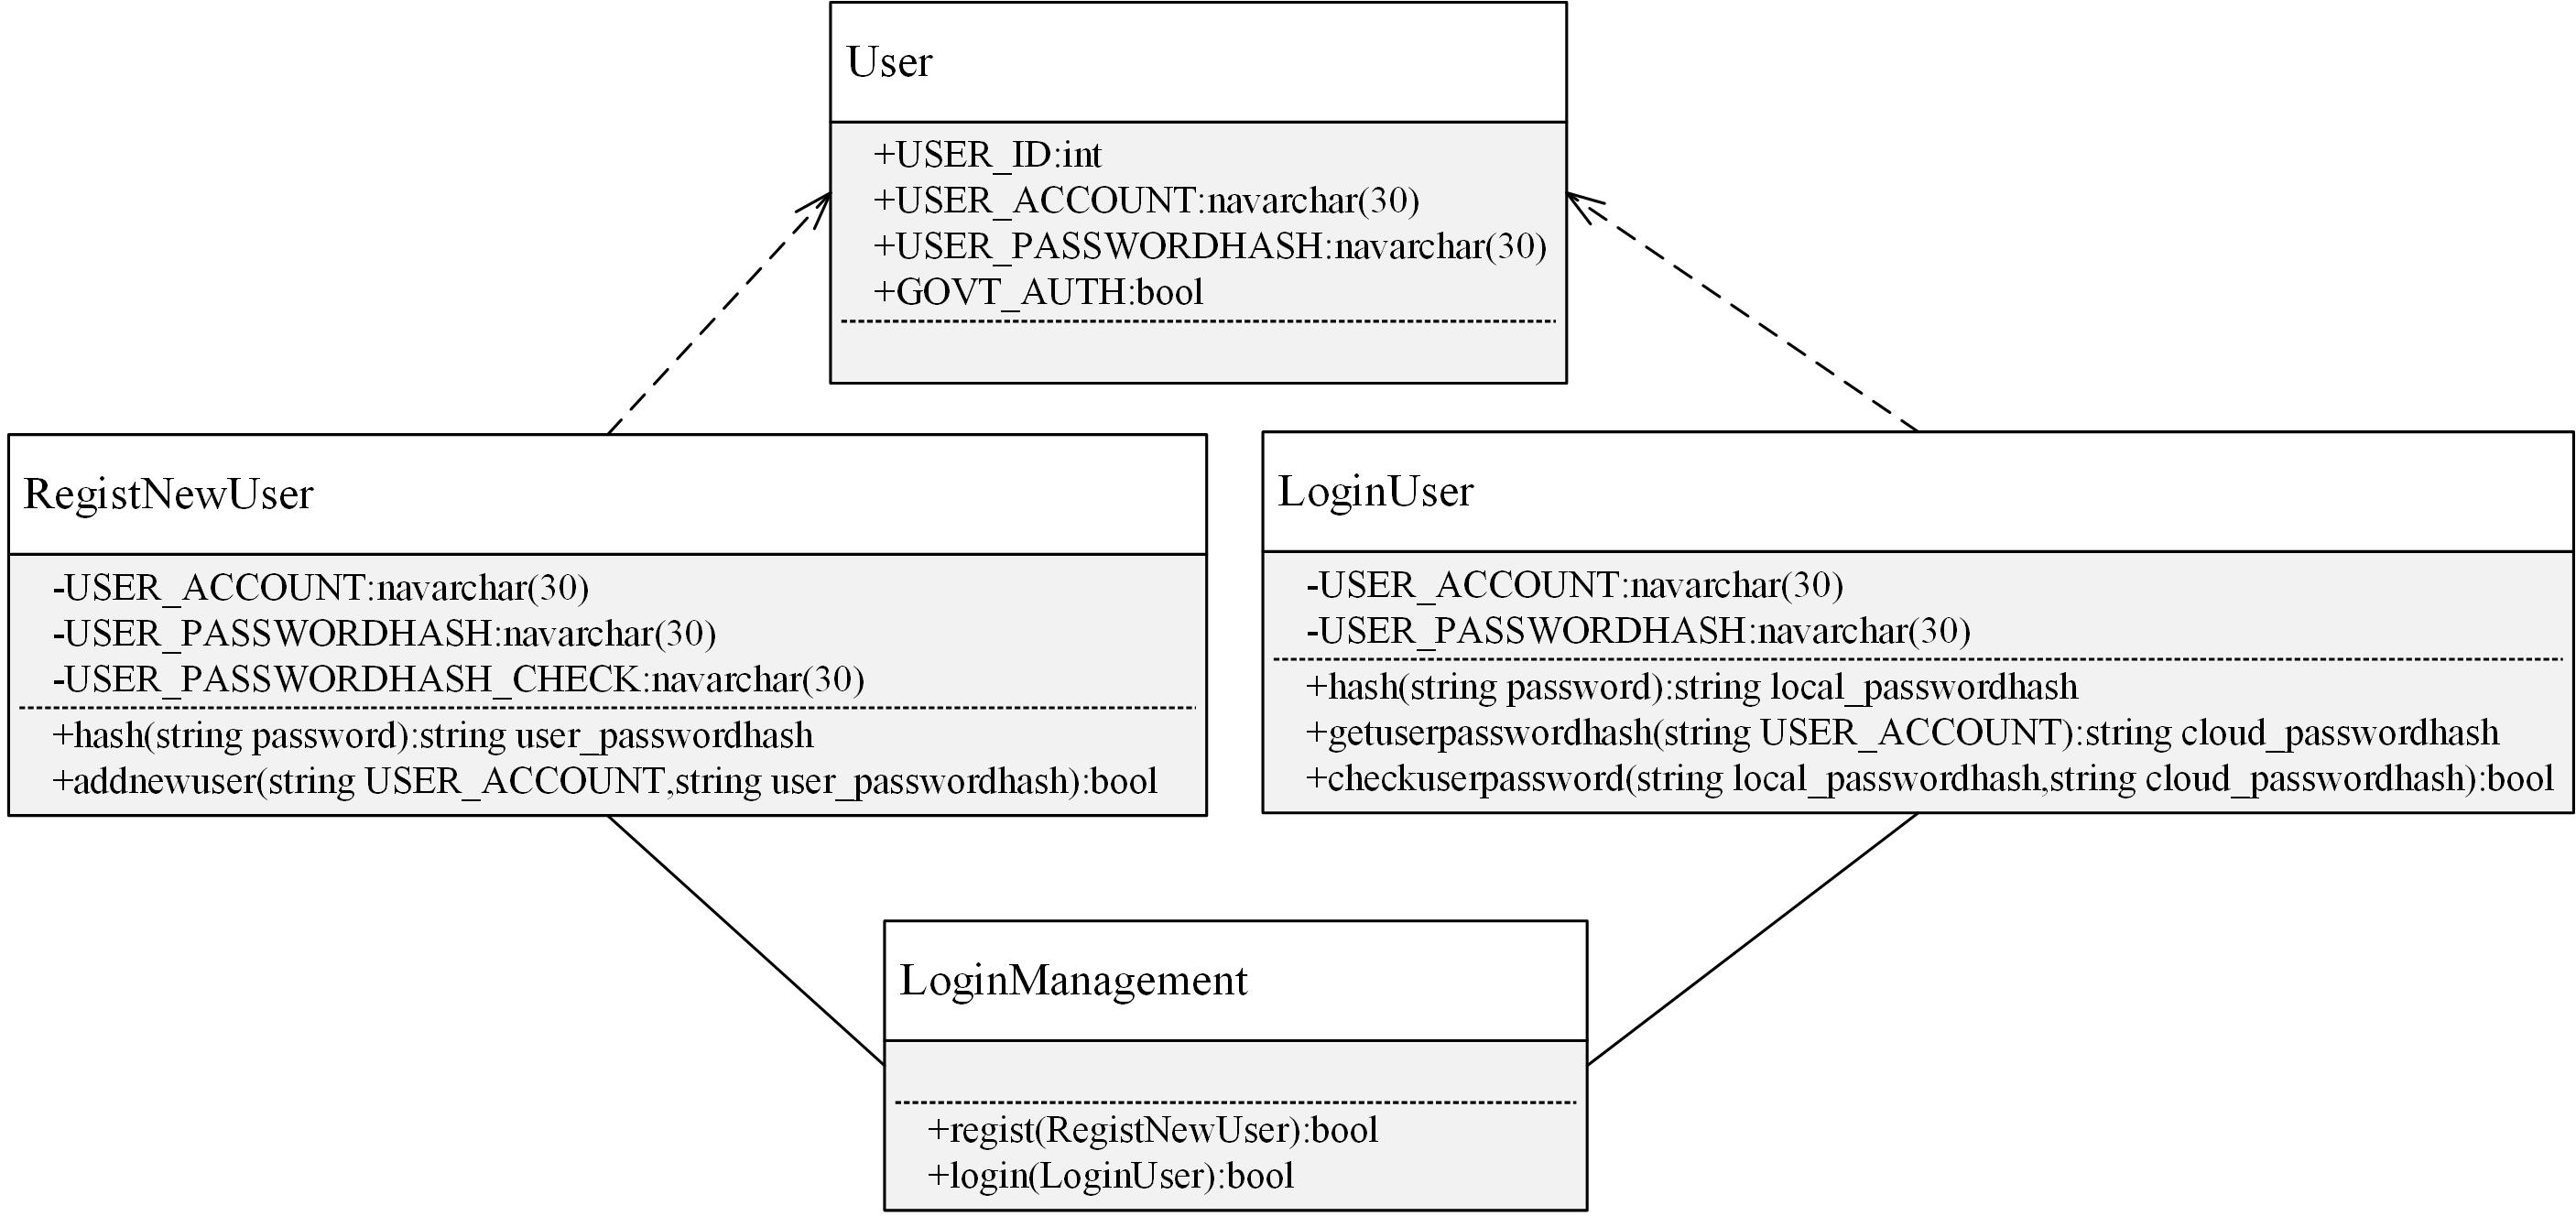
\includegraphics[width = 1\textwidth]{c3.pdf}
		\caption{用户注册与登入模块类图}\label{c3}
	\end{figure}

	图\ref{time1}为职工与商家注册时序图,以下为流程说明:

	\begin{figure}[!htbp]
		\centering
		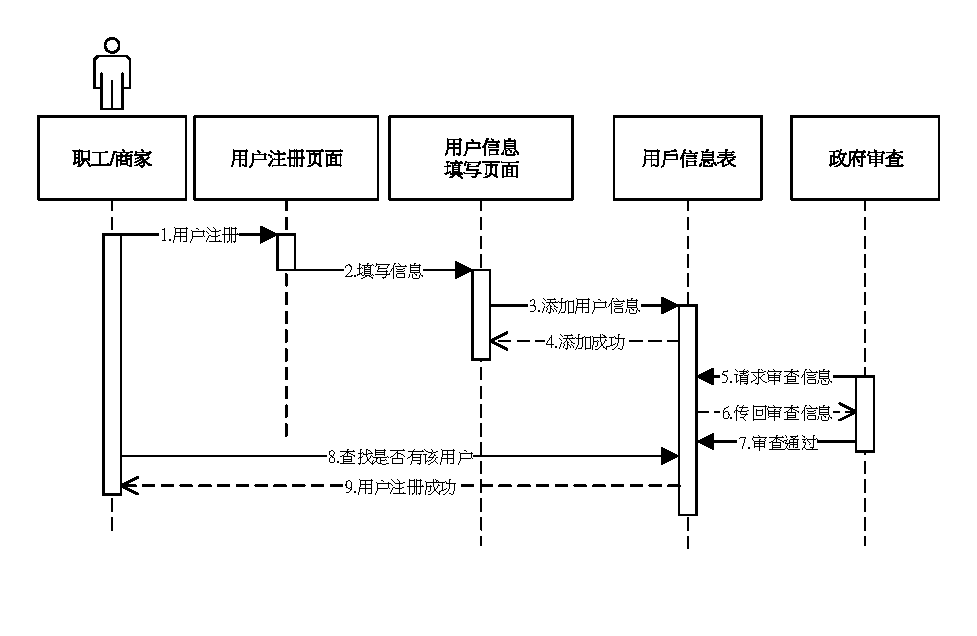
\includegraphics[width = 0.9\textwidth]{time1.pdf}
		\caption{职工与商家注册时序图}\label{time1}
	\end{figure}

	\begin{enumerate}
	\item 首先职工或是商家前往用户注册页面。
	\item 前往用户信息填写页面填写用户帐户信息以及用户密码。
	\item 完成填写后,为了提升用户密码信息安全,将用户密码以哈希算法计算后以密码哈希值保存。将填写完的帐号信息以及密码哈希值提交到用户信息表。
	\item 用户信息表则传回添加成功。届时的用户信息已经存储到用户信息表内但是尚未被激活,需要等待政府进行审查。
	\item 政府向用户信息请求表拿取所有还未被激活的用户信息。
	\item 数据库中的用户信息表传回政府请求的用户信息清单。
	\item 政府进行用户审查,在完成用户审查后,则向用户信息表内输入审查通过。
	\item 此时,用户再次访问用户信息表当中用户帐号是否已经激活成功。
	\item 用户信息表回传已经验证通过。
	\end{enumerate}


\subsubsection{(二)商家产品管理模块}
商家的运营需要管理本⾝所需贩售的商品。在商家完成注册⽤⼾帐号并且通过政府审核之后,便可查看所有的产品,近⼀步可以透过产品管理模块添加、修改以及删除商家商品。图\ref{c2}为商家产品管理类图,其中StoreProductManagement 类中有四个⽅法需要实现,分别为显⽰商家信息的showstoreinfo() ⽅法、显⽰商家产品信息的showstoreproductinfo() ⽅法、显⽰产品信息的showproductinfo() 方法以及修改商家产品信息的edit()⽅法。其中StoreProductCompare 类与EditStoreProduct 类需要向StoreProduct 类请求商家产品信息,StoreProductCompare 类中的compare() ⽅法是向商家产品信息表取得与STORE\_ID 相符的所有相关商家产品。EditStoreProduct 类中的addstoreproduct() ⽅法、editstoreproduct() ⽅法、以及deletestoreproduct() ⽅法分别为添加、修改、以及删除商家产品信息。StoreCompare 类中的compare() ⽅法是向Store 类请求与STORE\_ID 相符的商家信息。

	\begin{figure}[!htbp]
		\centering
		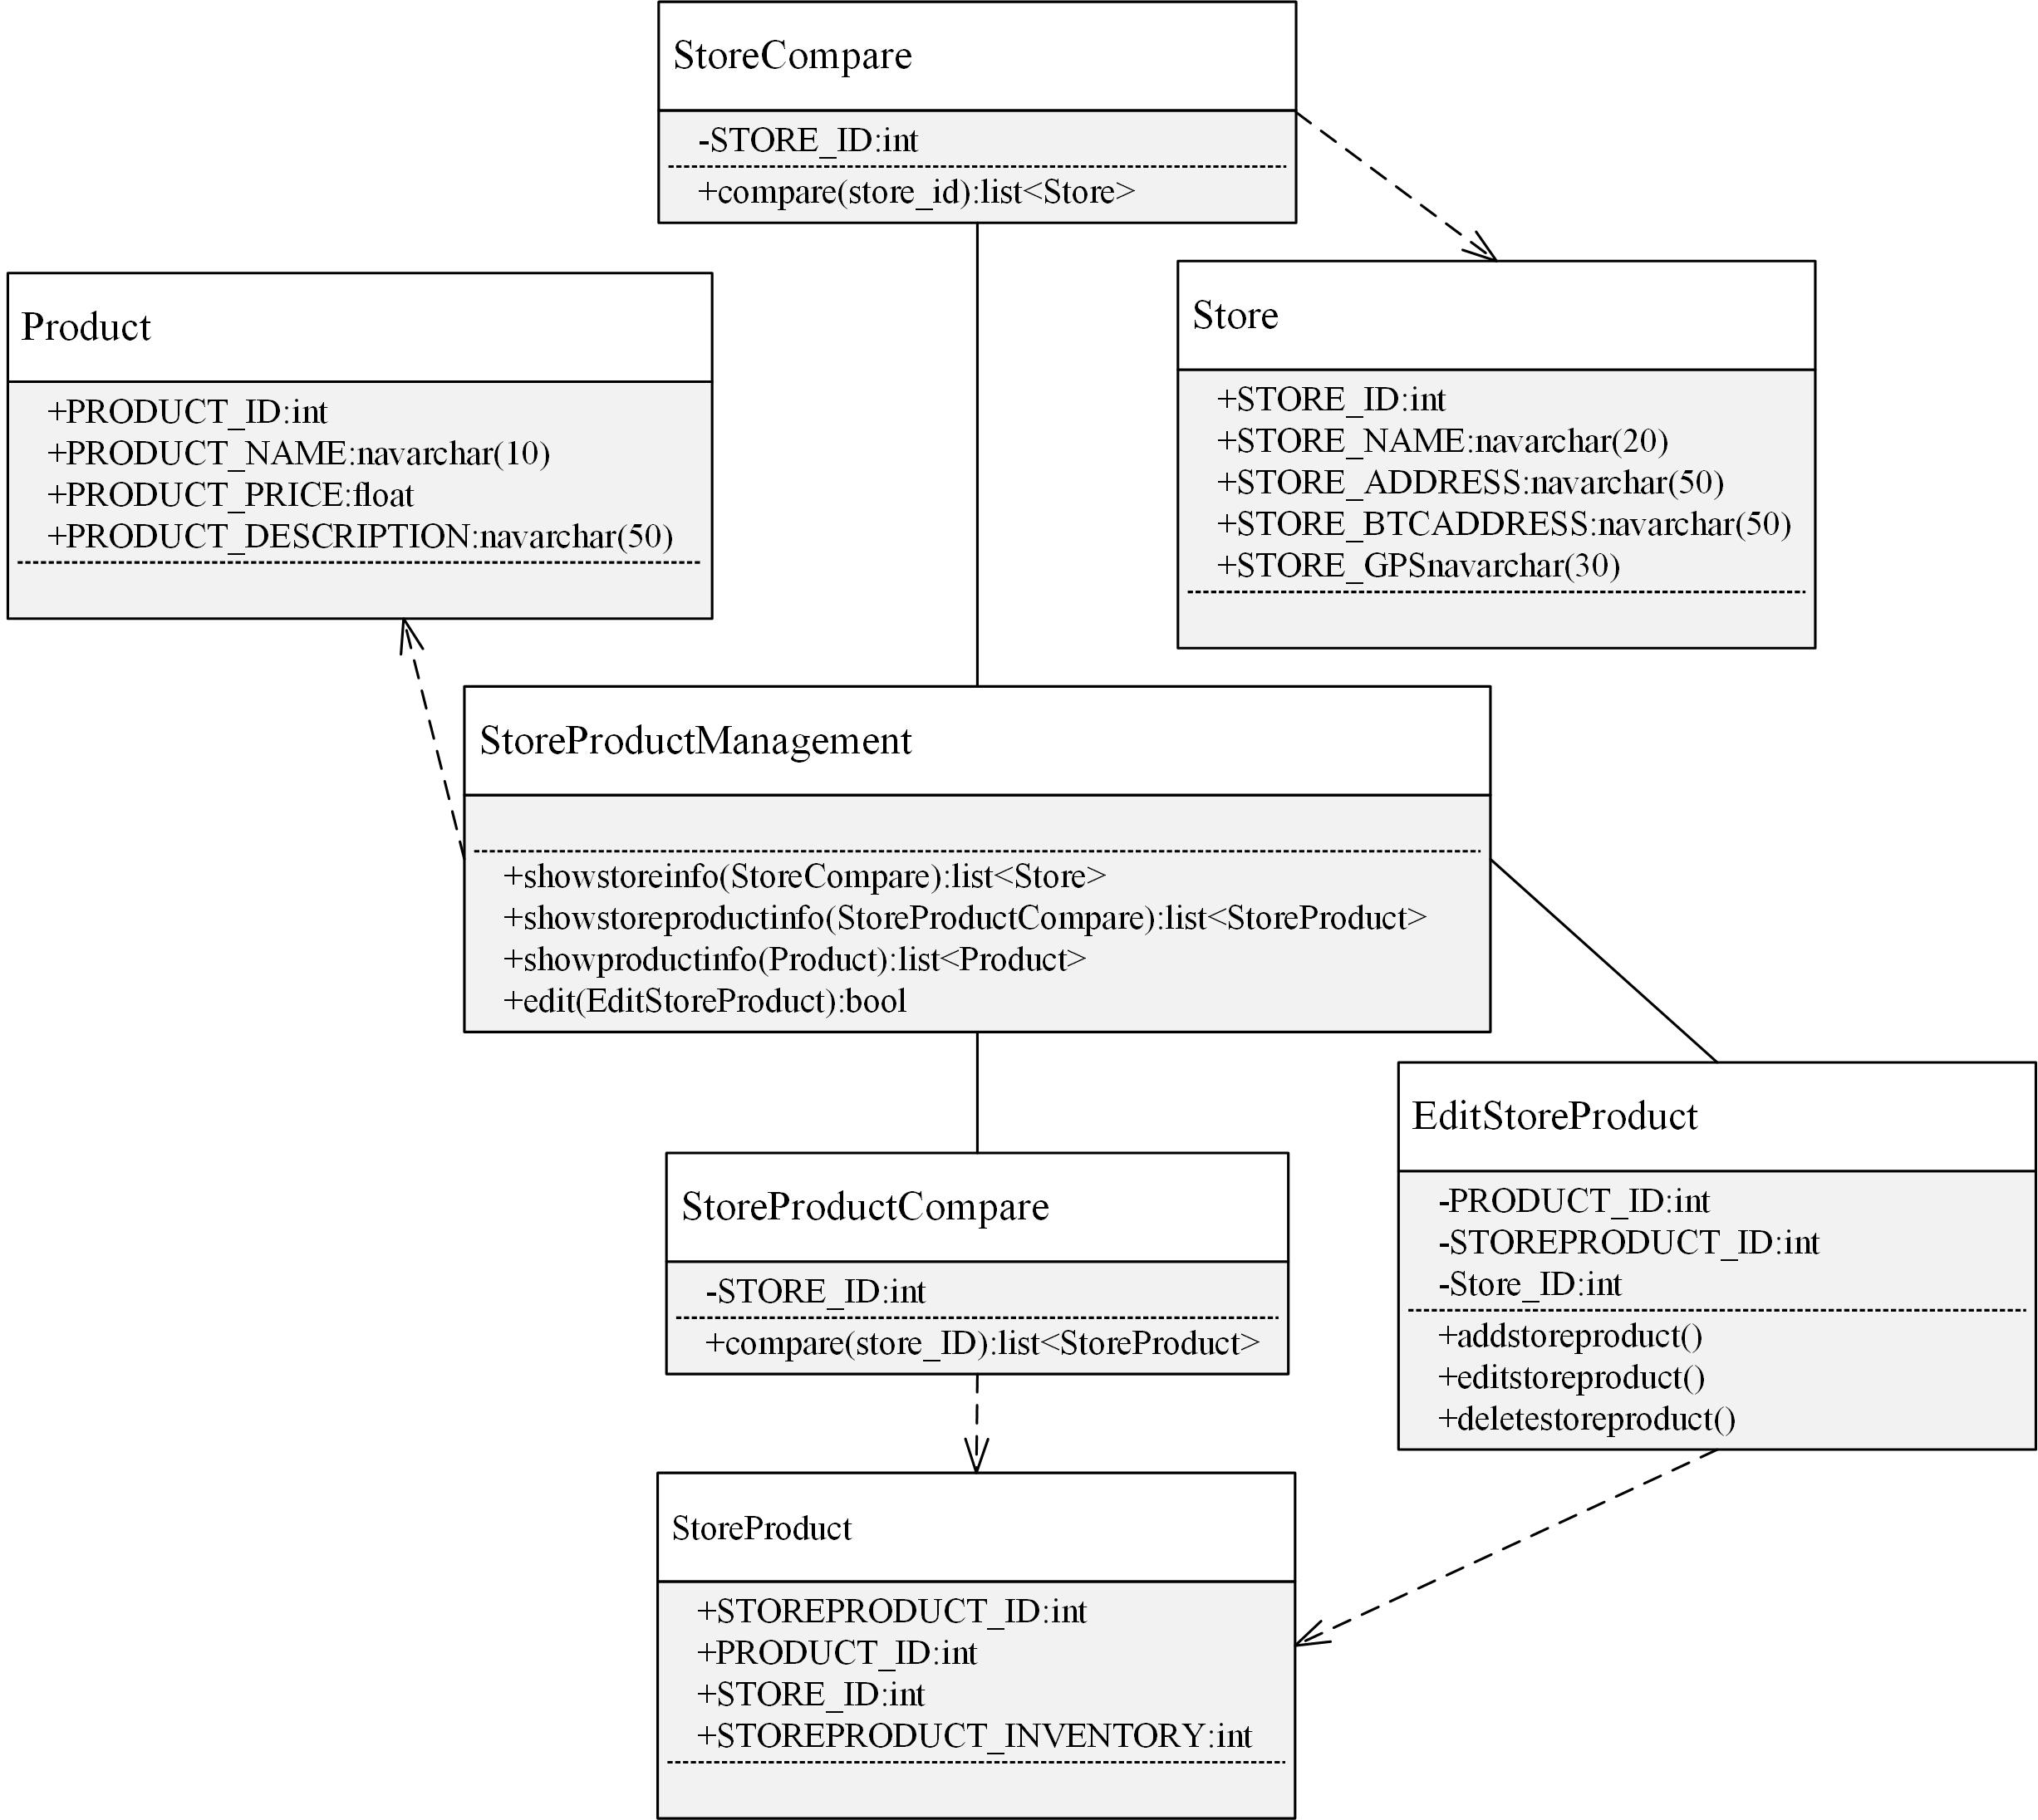
\includegraphics[width = 0.95\textwidth]{c2.pdf}
		\caption{商家产品管理类图}\label{c2}
	\end{figure}

	图\ref{time3}为商家产品管理时序图,以下为流程说明:

	\begin{figure}[!htbp]
		\centering
		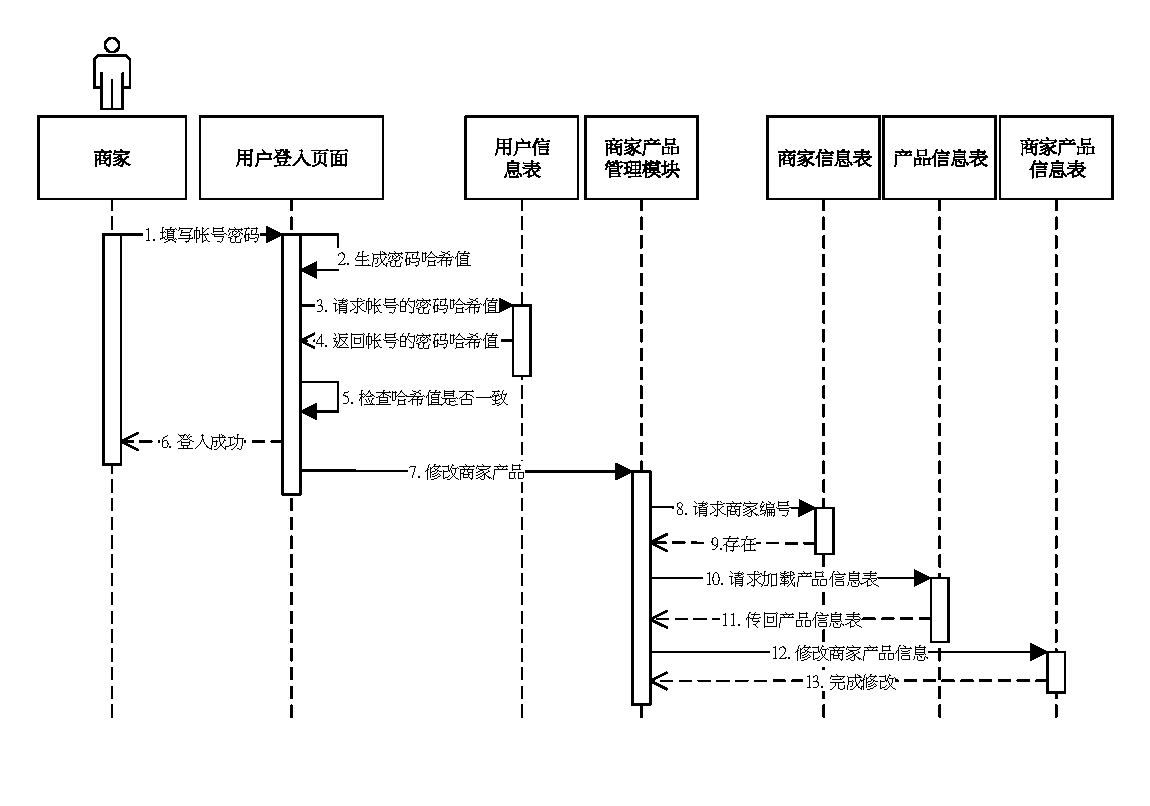
\includegraphics[width = 0.95\textwidth]{time3.pdf}
		\caption{商家产品管理时序图}\label{time3}
	\end{figure}

	\begin{enumerate}
	\item 商家在完成用户注册后并完成政府的审核之后,便可填写用户帐户与用户密码到登入页面。
	\item 登入页面会将用户提交之密码透过哈希算法生成密码哈希值。
	\item 用户登入页面向用户信息表询问该用户帐号的密码哈希值。
	\item 用户信息表将该帐户的密码哈希值传回给用户登入页面保存。
	\item 用户页面将本地密码哈希值和从数据库信息表中请求保存的密码哈希值进行比对是否相同。
	\item 倘若本地与数据库中的哈希值一致,则为登入成功。
	\item 登入成功后商家即可进入商家产品管理模块。
	\item 为确认欲修改的商家是否存在,所以向数据库中的商家信息表请求该商家编号是否存在。
	\item 商家信息表传回存在的信息。
	\item 向数据库中的产品信息表当中请求所有的产品信息。
	\item 产品信息表回传所有的产品信息。
	\item 此时商家已经确认商家信息是否存在,且已经取得所有的产品信息。商家向商家产品信息表提交商家要增加的产品编号以及商家本身的商家编号,此时生成商家产品编号。
	\item 商家信息表在完成添加商家产品信息之后,传回添加成功的信息到商家产品管理模块。
	\end{enumerate}


\subsubsection{(三)职工管理模块}
商家需要职⼯进⾏商家的运营。在商家⽤⼾完成政府审查之后,便可以进⼊职⼯管理模块,透过提交⽤⼾编号以及商家编号添加、修改以及删除职⼯信息。图\ref{c1}为职⼯管理模块类图,StaffManagement 类当中有四种⽅法,前三种分别为显⽰与该商家STORE\_ID 相符的完整信息showstore() ⽅法、显⽰符合该商家STORE\_ID 职⼯信息的showstorestaff() ⽅法、显⽰⽤⼾编号的showuser() ⽅法。而在第四种edit()方法中,UserCompare 类需要向User 类提取⽤⼾相关信息实现查找,StoreCompare 类需要向Store 类请求商家信相关信息,其中EditStoreStaff 类与StoreStaffCompare 类需要使⽤到Staff 类修改职⼯信息表的内容,EditStoreStaff 类中的addstaff()、editstaff() 以及deletestaff() ⽅法分别为添加、修改以及删除职⼯,StoreStaffCompare 类中的compare() ⽅法是取得符合STORE\_ID 的所有职⼯信息。

	\begin{figure}[!htbp]
		\centering
		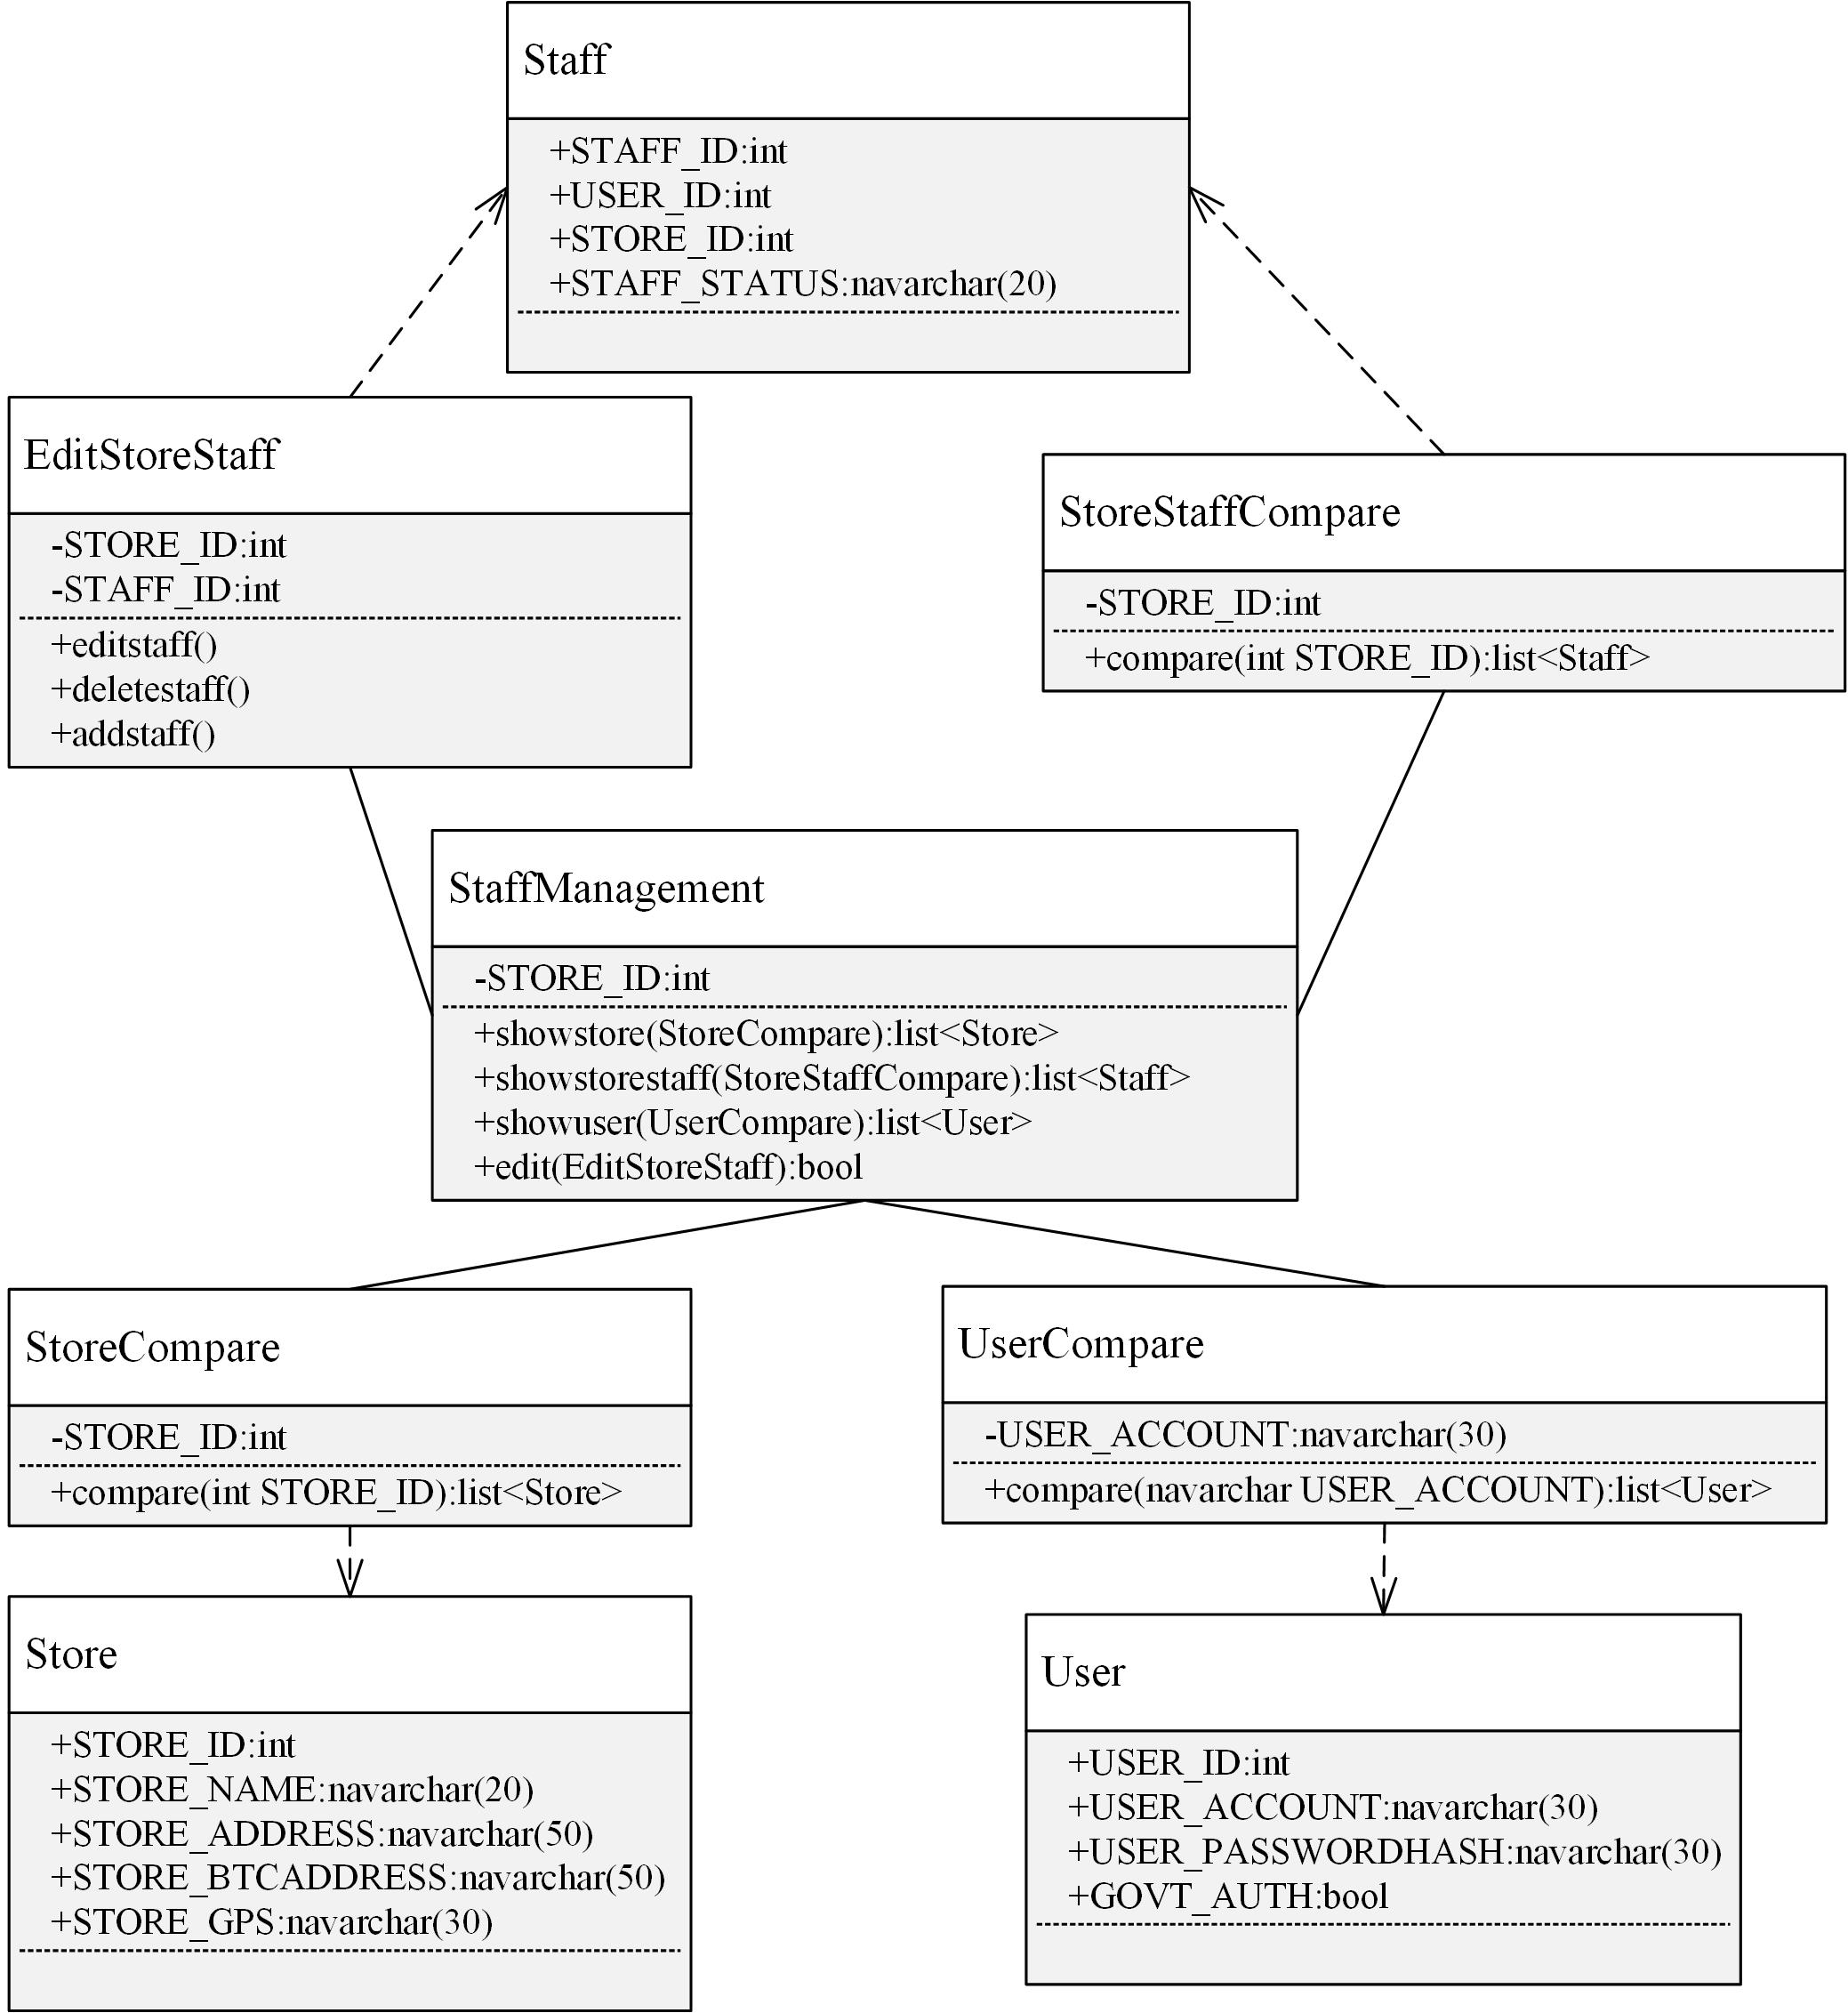
\includegraphics[width = 0.8\textwidth]{c1.pdf}
		\caption{职工管理模块类图}\label{c1}
	\end{figure}

	

	图\ref{time2}为商家职工管理时序图,以下为流程说明:

	\begin{figure}[!htbp]
		\centering
		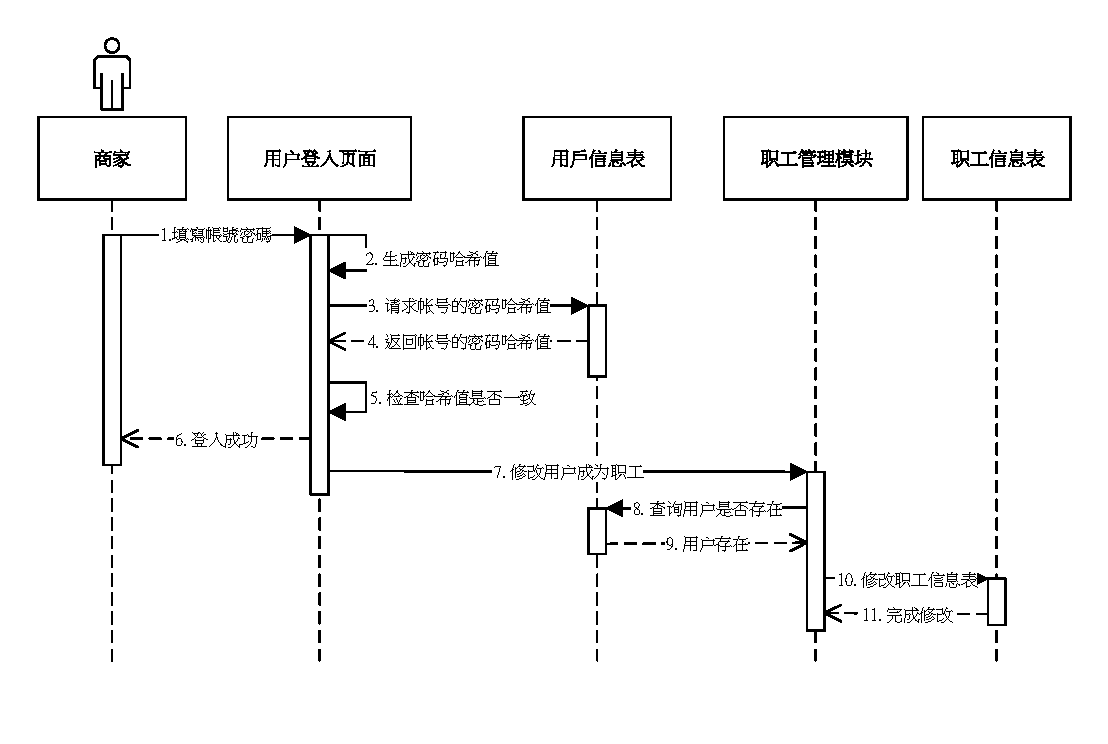
\includegraphics[width = 0.95\textwidth]{time2.pdf}
		\caption{职工管理时序图}\label{time2}
	\end{figure}

	\begin{enumerate}
	\item 商家前往用户登入页面输入用户帐号密码。
	\item 用户登入页面自动使用哈希算法将用户密码转换成密码哈希值。
	\item 用户登入页面向数据库中的用户信息表请求该用户帐号的密码哈希值。
	\item 数据库用户信息表回传用户密码哈希值。
	\item 用户登入页面比对本地端的用户密码哈希值与数据库中的密码哈希值是否一致。
	\item 倘若数据库中的密码哈希值与用户登入页面生成的密码哈希值一致,则登入成功。
	\item 商家提交商家编号以及欲添加的用户编号。
	\item 职工管理模块向用户信息表查找该用户是否存在。
	\item 用户信息表传回用户存在信息。
	\item 职工管理模块向数据库中的职工信息表提交用户编号、商家编号以及职工编号修改职工信息。
	\item 职工信息表传回修改完成。
	\end{enumerate}

\subsubsection{(四)商家交易管理模块}
在⽤⼾完成注册后且在商家将该⽤⼾加⼊成为公司职⼯后,该职⼯可以透过⽤⼾帐号进⼊到商家交易管理模块,该模块为手持移动装置的应⽤程序。在进⼊到本模块后会⾃动加载商家商品、商家信息以及职⼯信息,制成⼀个基于区块链加密货币的移动收银机,可以扫描带有RFID 标签的商家产品,创建交易后等待⽤⼾交易管理模块读取以及验证交易是否完成的信息。图5.8为商家交易管理模块类图,在StoreTransactionManagement 类当中有五个⽅法,分别为显⽰所有的商家产品信息的showstoreproduct() ⽅法、显⽰职⼯信息的showstorestaff()⽅法、显⽰商家信息的showstore() ⽅法、检查交易是否完成的check() ⽅法以及透过NFC 传输协议传输信息的nfc() ⽅法。StoreCompare 类中的compare() ⽅法是向Store类取得与STORE\_ID 相符的商家信息,StoreProductCompare 类中的compare() ⽅法是向StoreProduct 类请求与STORE\_ID 相符的所有商家产品信息。StoreStaffCompare 类中的compare() ⽅法是向Staff 类中请与USER\_ID 相符的职⼯信息。在NFCMessage 类中有两个⽅法,receivenfcmessage() 方法⽅法使得商家可以快速的扫描商品的RFID 标签,sendnfcmessage() 方法⽅法使得职⼯在创建完交易清单后可以将交易信息发送给顾客。CheckTx 类中有两个⽅法,分别为取得于Tx 类中交易信息的compare() ⽅法,以及getcheck()⽅法是检查该笔交易的CHECK 值是否已经在Tx 类中被修改为"1",倘若被修改为"1"则表示该笔交易已经被写⼊区块链中。在本模块要做到验证⽐特币交易是否已经被存储在⽐特币区块链当中,必须使⽤BlockchainExplorer 类中的getblockchain() ⽅法取得所有区块链相关的信息,再透过getbitcointx() ⽅法取得该笔⽐特币交易的状态以及详细信息。Tx 类中可以调⽤txcheck() ⽅法对BlockchainExplorer 类检查该笔交易是否已经进⼊了区块链,如果已经进⼊区块链,则将相关的交易信息的CHECK 值修改为"1"。值得⼀提的是,在此将CHECK 值修改为"1"的标准,为该笔交易进⼊区块链的时间。由于⽐特币区块链的⽣成速度平均为每⼗分钟⼀块,这将使得交易确认速度不够即时。


	\begin{figure}[!htbp]
		\centering
		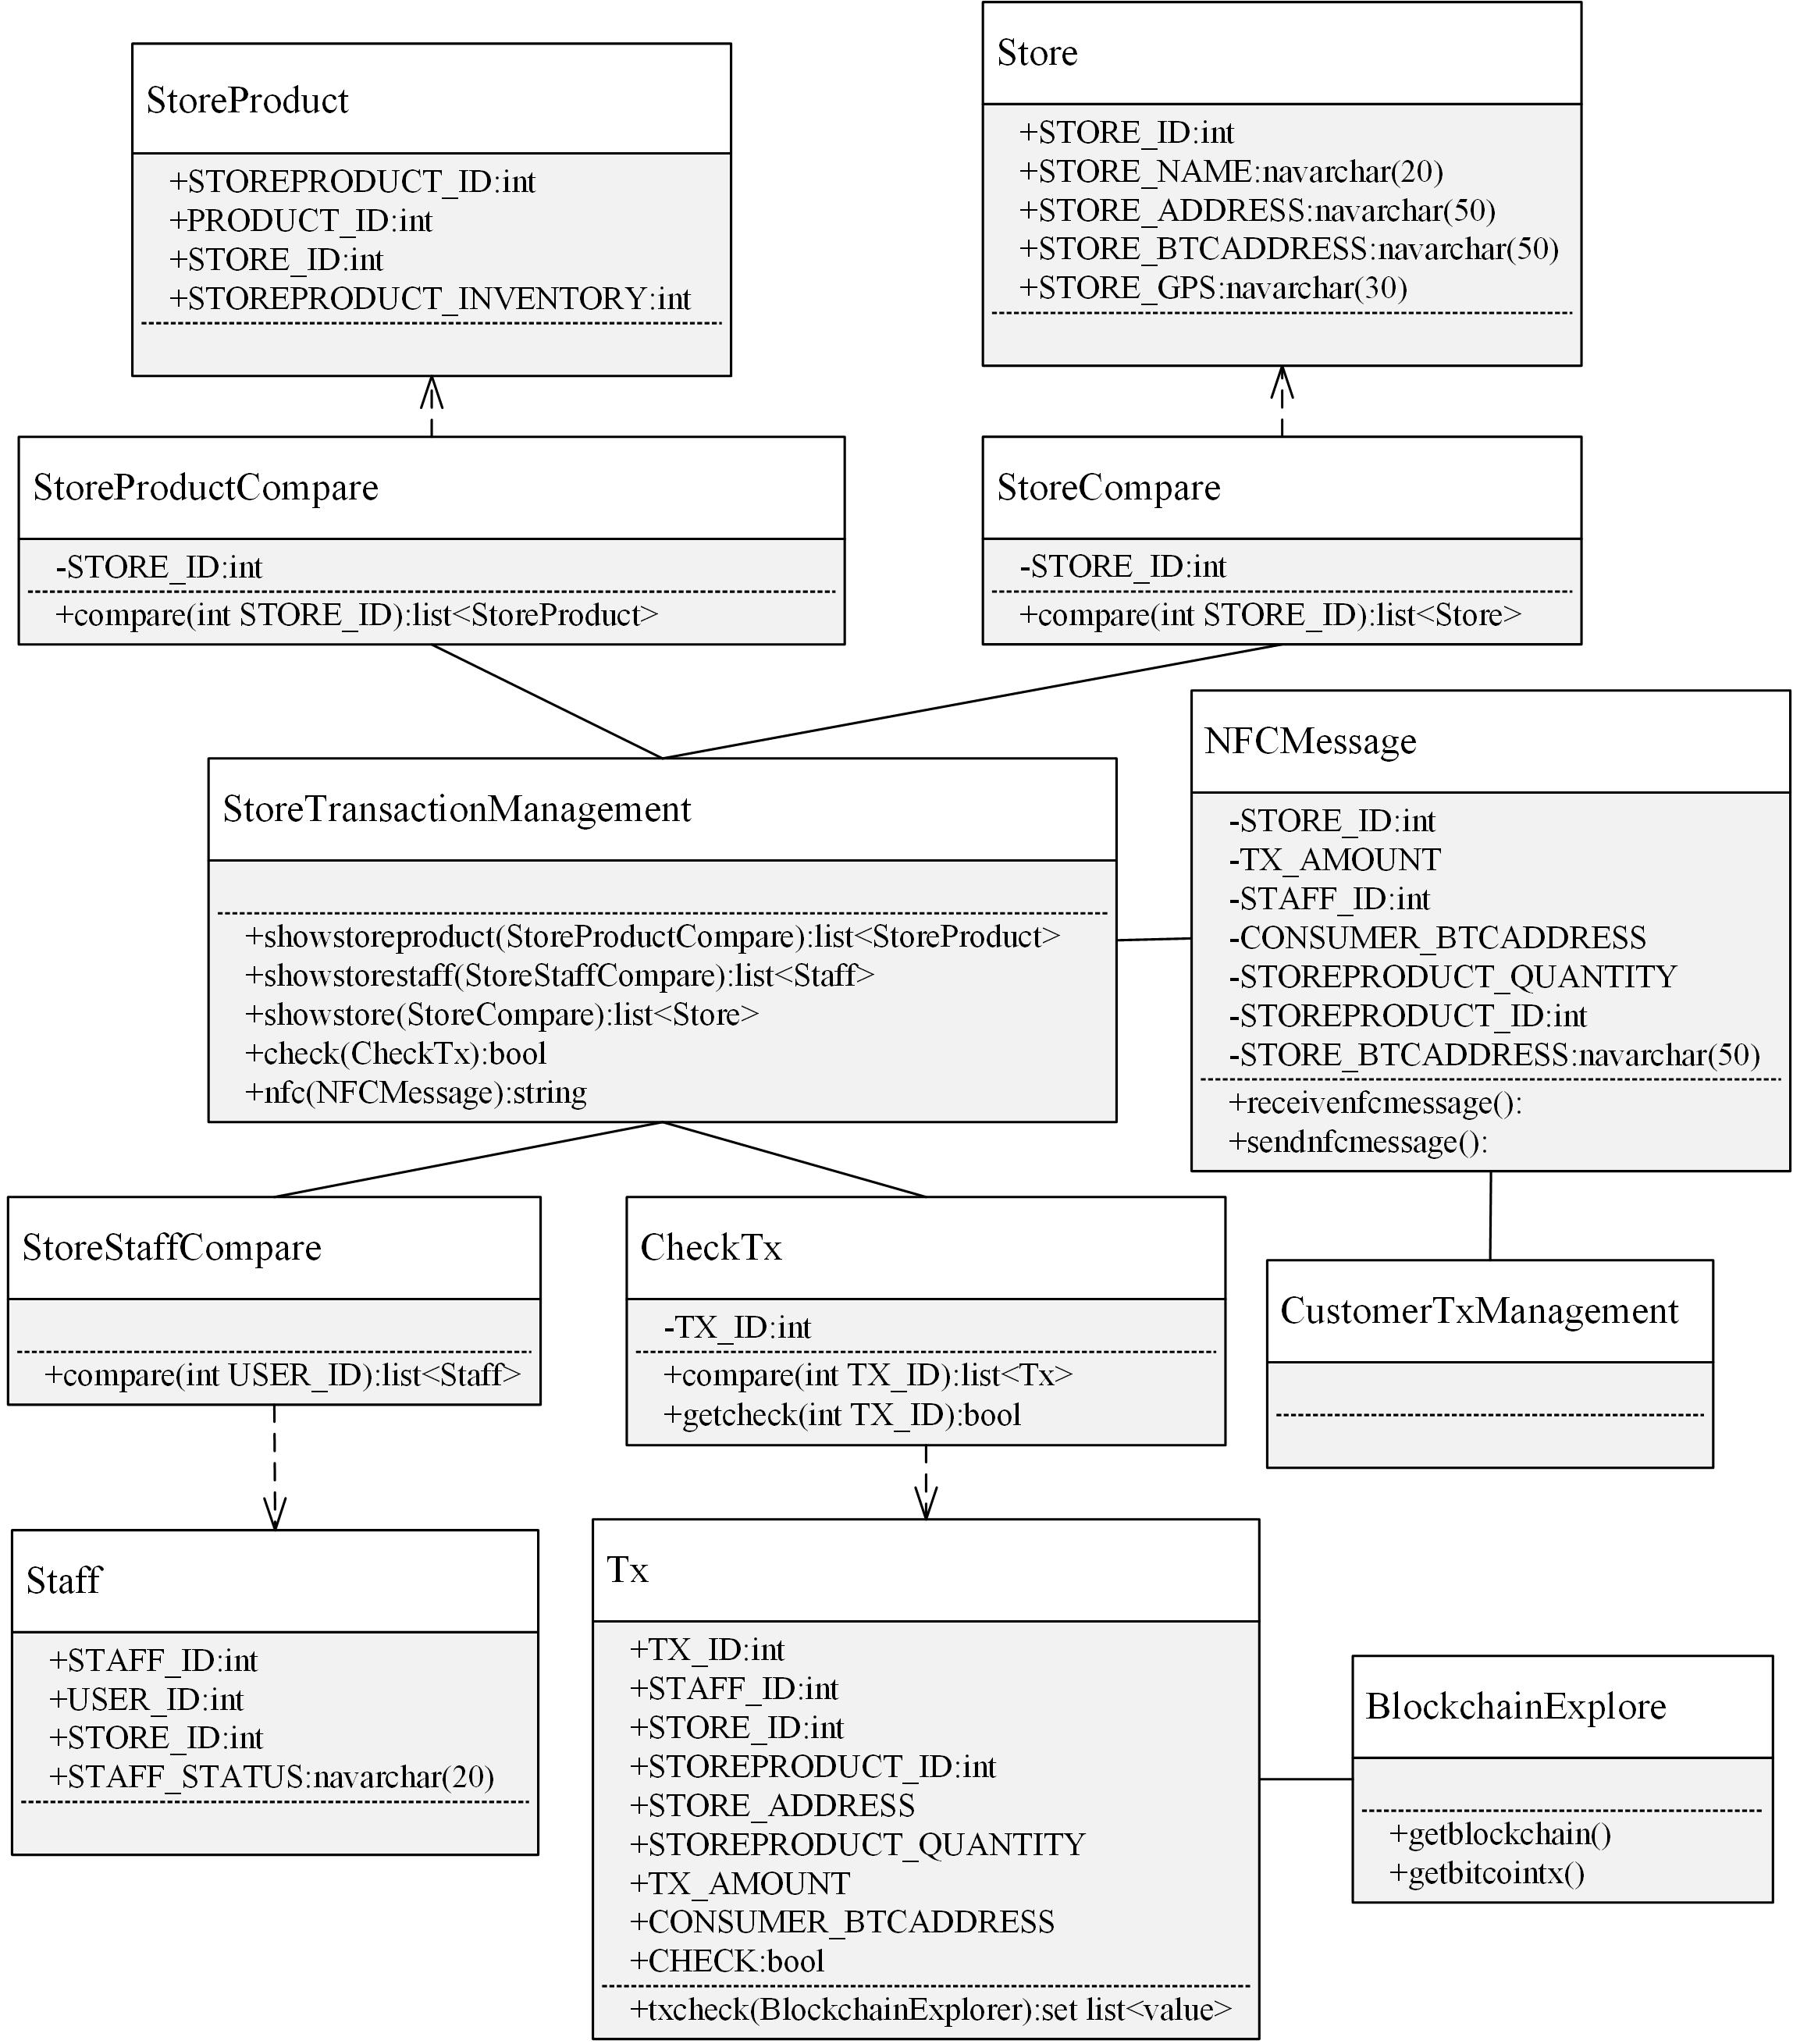
\includegraphics[width = 0.9\textwidth]{c5.pdf}
		\caption{商家交易管理模块类图}\label{c5}
	\end{figure}


图\ref{time4}为商家交易管理时序图,以下为流程说明:

	\begin{figure}[!htbp]
		\centering
		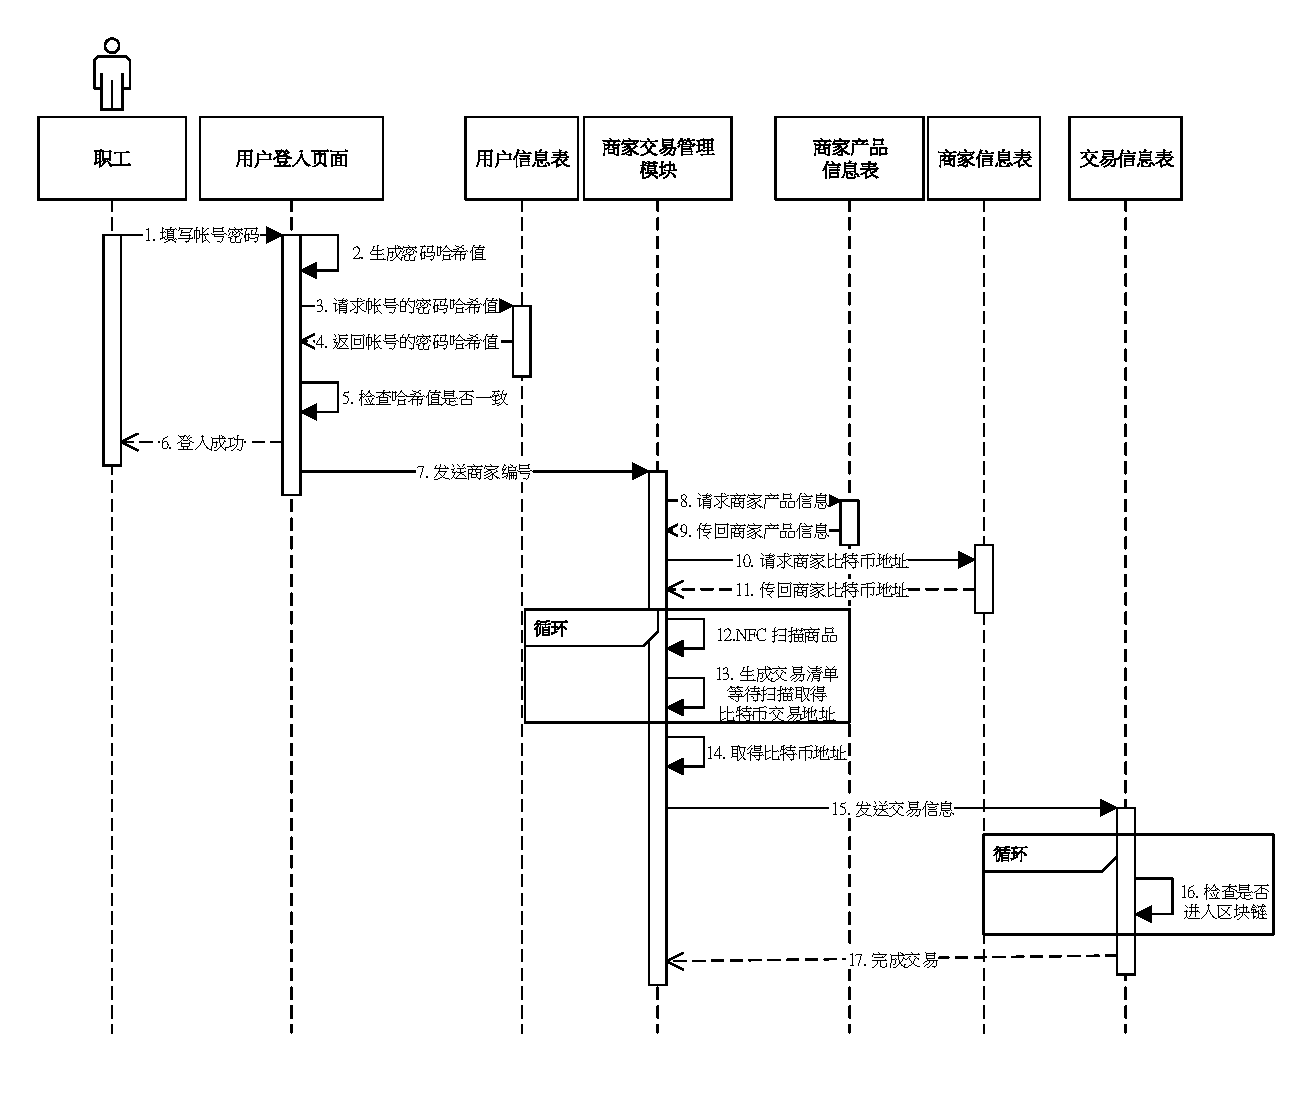
\includegraphics[width = 1\textwidth]{time4.pdf}
		\caption{商家交易管理时序图}\label{time4}
	\end{figure}

	\begin{enumerate}
	\item 首先职工填写用户的帐号密码到用户登入页面。
	\item 用户登入页面模块将用户填写的密码透过哈希算法生成本地端的用户密码哈希值。
	\item 将用户填写的帐号发送到用户信息表请求远程的用户密码哈希值以及商家编号。
	\item 用户信息表传回远程的用户密码哈希值。
	\item 用户登入页面模块进行本地用户密码哈希值和远程用户密码哈希值比对是否一样。
	\item 倘若一致则登入成功。
	\item 此时用户登入页面向商家交易管理模块发送商家编号的信息,商家交易管理模块将信息保存。
	\item 商家交易管理模块向商家产品信息表请求与商家编号相关的所有商家产品信息。
	\item 商家产品信息表传回所有与商家相关的商家产品信息至商家交易管理模块。
	\item 商家交易管理模块向商家信息表请求商家比特币地址信息。
	\item 商家信息表将商家比特币地址信息传回到商家交易管理模块。
	\item 商家产品信息表将所有与商家编号有关的商家产品信息传回到商家交易管理模块,此时商家交易管理模块已经有完整的商家产品信息以及商家信息。将带有RFID标签的商品透过NFC线圈进行传感对应到相关的商家产品信息。
	\item 将产品信息创建交易清单显示在手持移动装置的屏幕上,等待顾客的手持设备进行感应,感应的同时会将交易清单以及商家比特币地址发送到顾客交易管理模块。

	\item 在感应的同时顾客交易管理模块会将比特币钱包模块中的比特币地址提交给商家交易管理模块。
	\item 商家交易管理模块发送信息至交易信息表查找该笔交易信息。
	\item 交易信息表不断的向区块链检视器查找该笔比特币交易是否已经被写入比特币区块链内,倘若写入区块链则将交易信息的CHECK信息由"0"改为"1"。
	\item 交易信息表传回该笔交易的CHECK已经为"1"则完成交易。
	
	\end{enumerate}

	在比特币系统中,使得一笔比特币交易得到比特币网络的认可,需要等待六个区块的交易验证,相当于需要费时60分钟的时间等待一个交易的完成,这使得比特币交易在商家进行小额交易造成很大的不便,因此为了在BTMS中改善此问题,便导入了基于Green Address钱包的多重签章算法,使得交易时间可以从60分钟的等待时间,缩短为一秒钟左右。图\ref{c7}为商家Government Green Address交易管理模块类图,在此模块类图中针对Tx类中添加ggatxcheck()方法,使得商家交易管理模块可以支持Government Green Address地址格式的辨别,当检测到为Government Green Address地址格式,将交易信息中的CHECK字段修改为"1",这使得比特币交易信息可以在平均一秒钟的时间得到交易确认,ggatxcheck()方法需要调用BlockchainExplorer类中的getblockchain()取得比特币区块链的信息以及getbitcointx()方法得到比特币交易信息。在GovernmentGreenaddressCheckTx类中提供compare()方法可以针对Government Green Address地址向Tx类查找相关信息以及ggatxcheck()方法检测该笔交易是否存储于交易信息中的CHECK值已经被修改为"1"。

	

	\begin{figure}[!htbp]
		\centering
		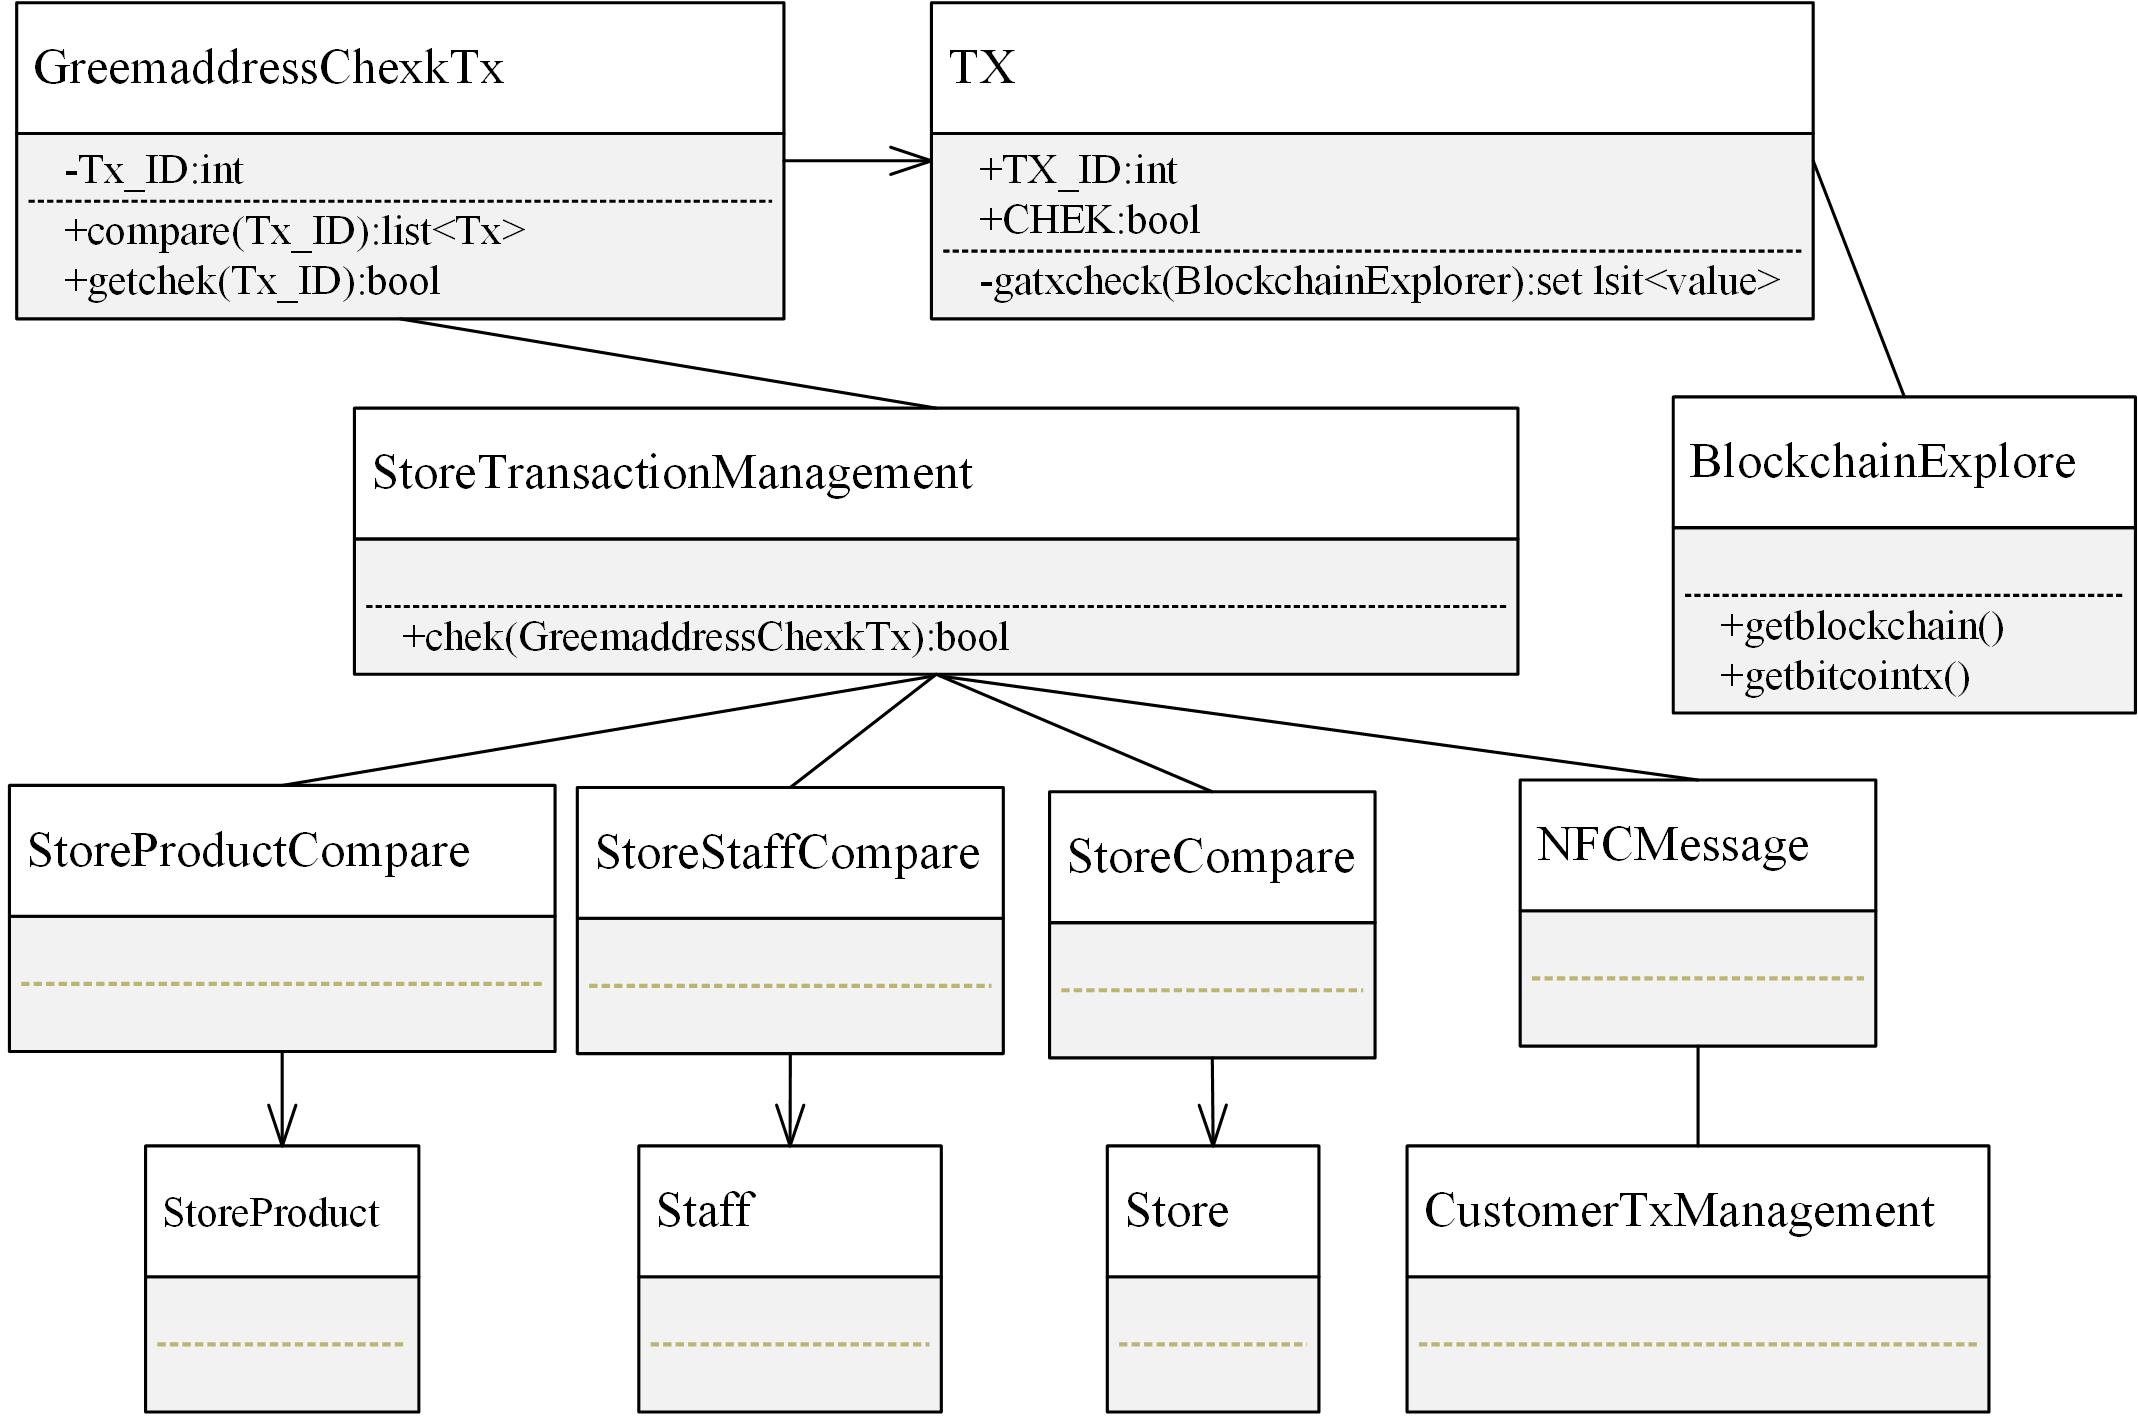
\includegraphics[width = 0.8\textwidth]{c7.pdf}
		\caption{商家Government Green Address交易管理模块类图}\label{c7}
	\end{figure}



\subsubsection{(五)顾客交易管理模块}
在本系统中顾客需要在手持移动端安装手持移动装置程序包括顾客交易管理模块,使得顾客手持移动装置可以支持比特币支付、查找过去的交易信息、以NFC通信协议接收商家交易管理模块创建的交易信息以及详细的商家商品信息。图\ref{c4}为顾客交易管理模块类图,在CustomerTxManagement 类中包括六个⽅法,分别为显⽰所有该⽤⼾拥有⽐特币交易信息相关的交易明细的showtx() ⽅法、取得交易信息后取得相对应的商家产品信息的showstoreproduct() ⽅法、检查于交易信息表中的交易信息CHECK 字段的值是否已经被填⼊"1"的check() ⽅法、发送详细的交易信息⾄交易信息表保存的sendtx2table()⽅法、透过NFC 协议接收于StoreTransactionManagement 类所创建的交易信息以及发送⽤⼾⽐特币地址的nfc() ⽅法,最后是控制⽐特币钱包的bitcoinpayment() ⽅法。CheckTx类中的getcheck() ⽅法可以向Tx 类询问该笔交易是否已经得到认证,TxCompare 类中的compare() ⽅法提供⽤⼾向交易信息表查找与⽤⼾交易信息相关的交易,TransferTx类中的sendtx() ⽅法是将顾客完成交易的交易信息提交到交易信息表,BitcoinPay 类使⽤pay() ⽅法⽀付⽐特币,NFCMessage 类中的receivenfcmessage() 和sendnfcmessage()分别为透过NFC 协议发送以及接收交易信息和顾客⽐特币地址。StoreProductCompare类则是向StoreProduct 类请求顾客手持移动装置中所有交易信息中相关的商家商品。

	\begin{figure}[!htbp]
		\centering
		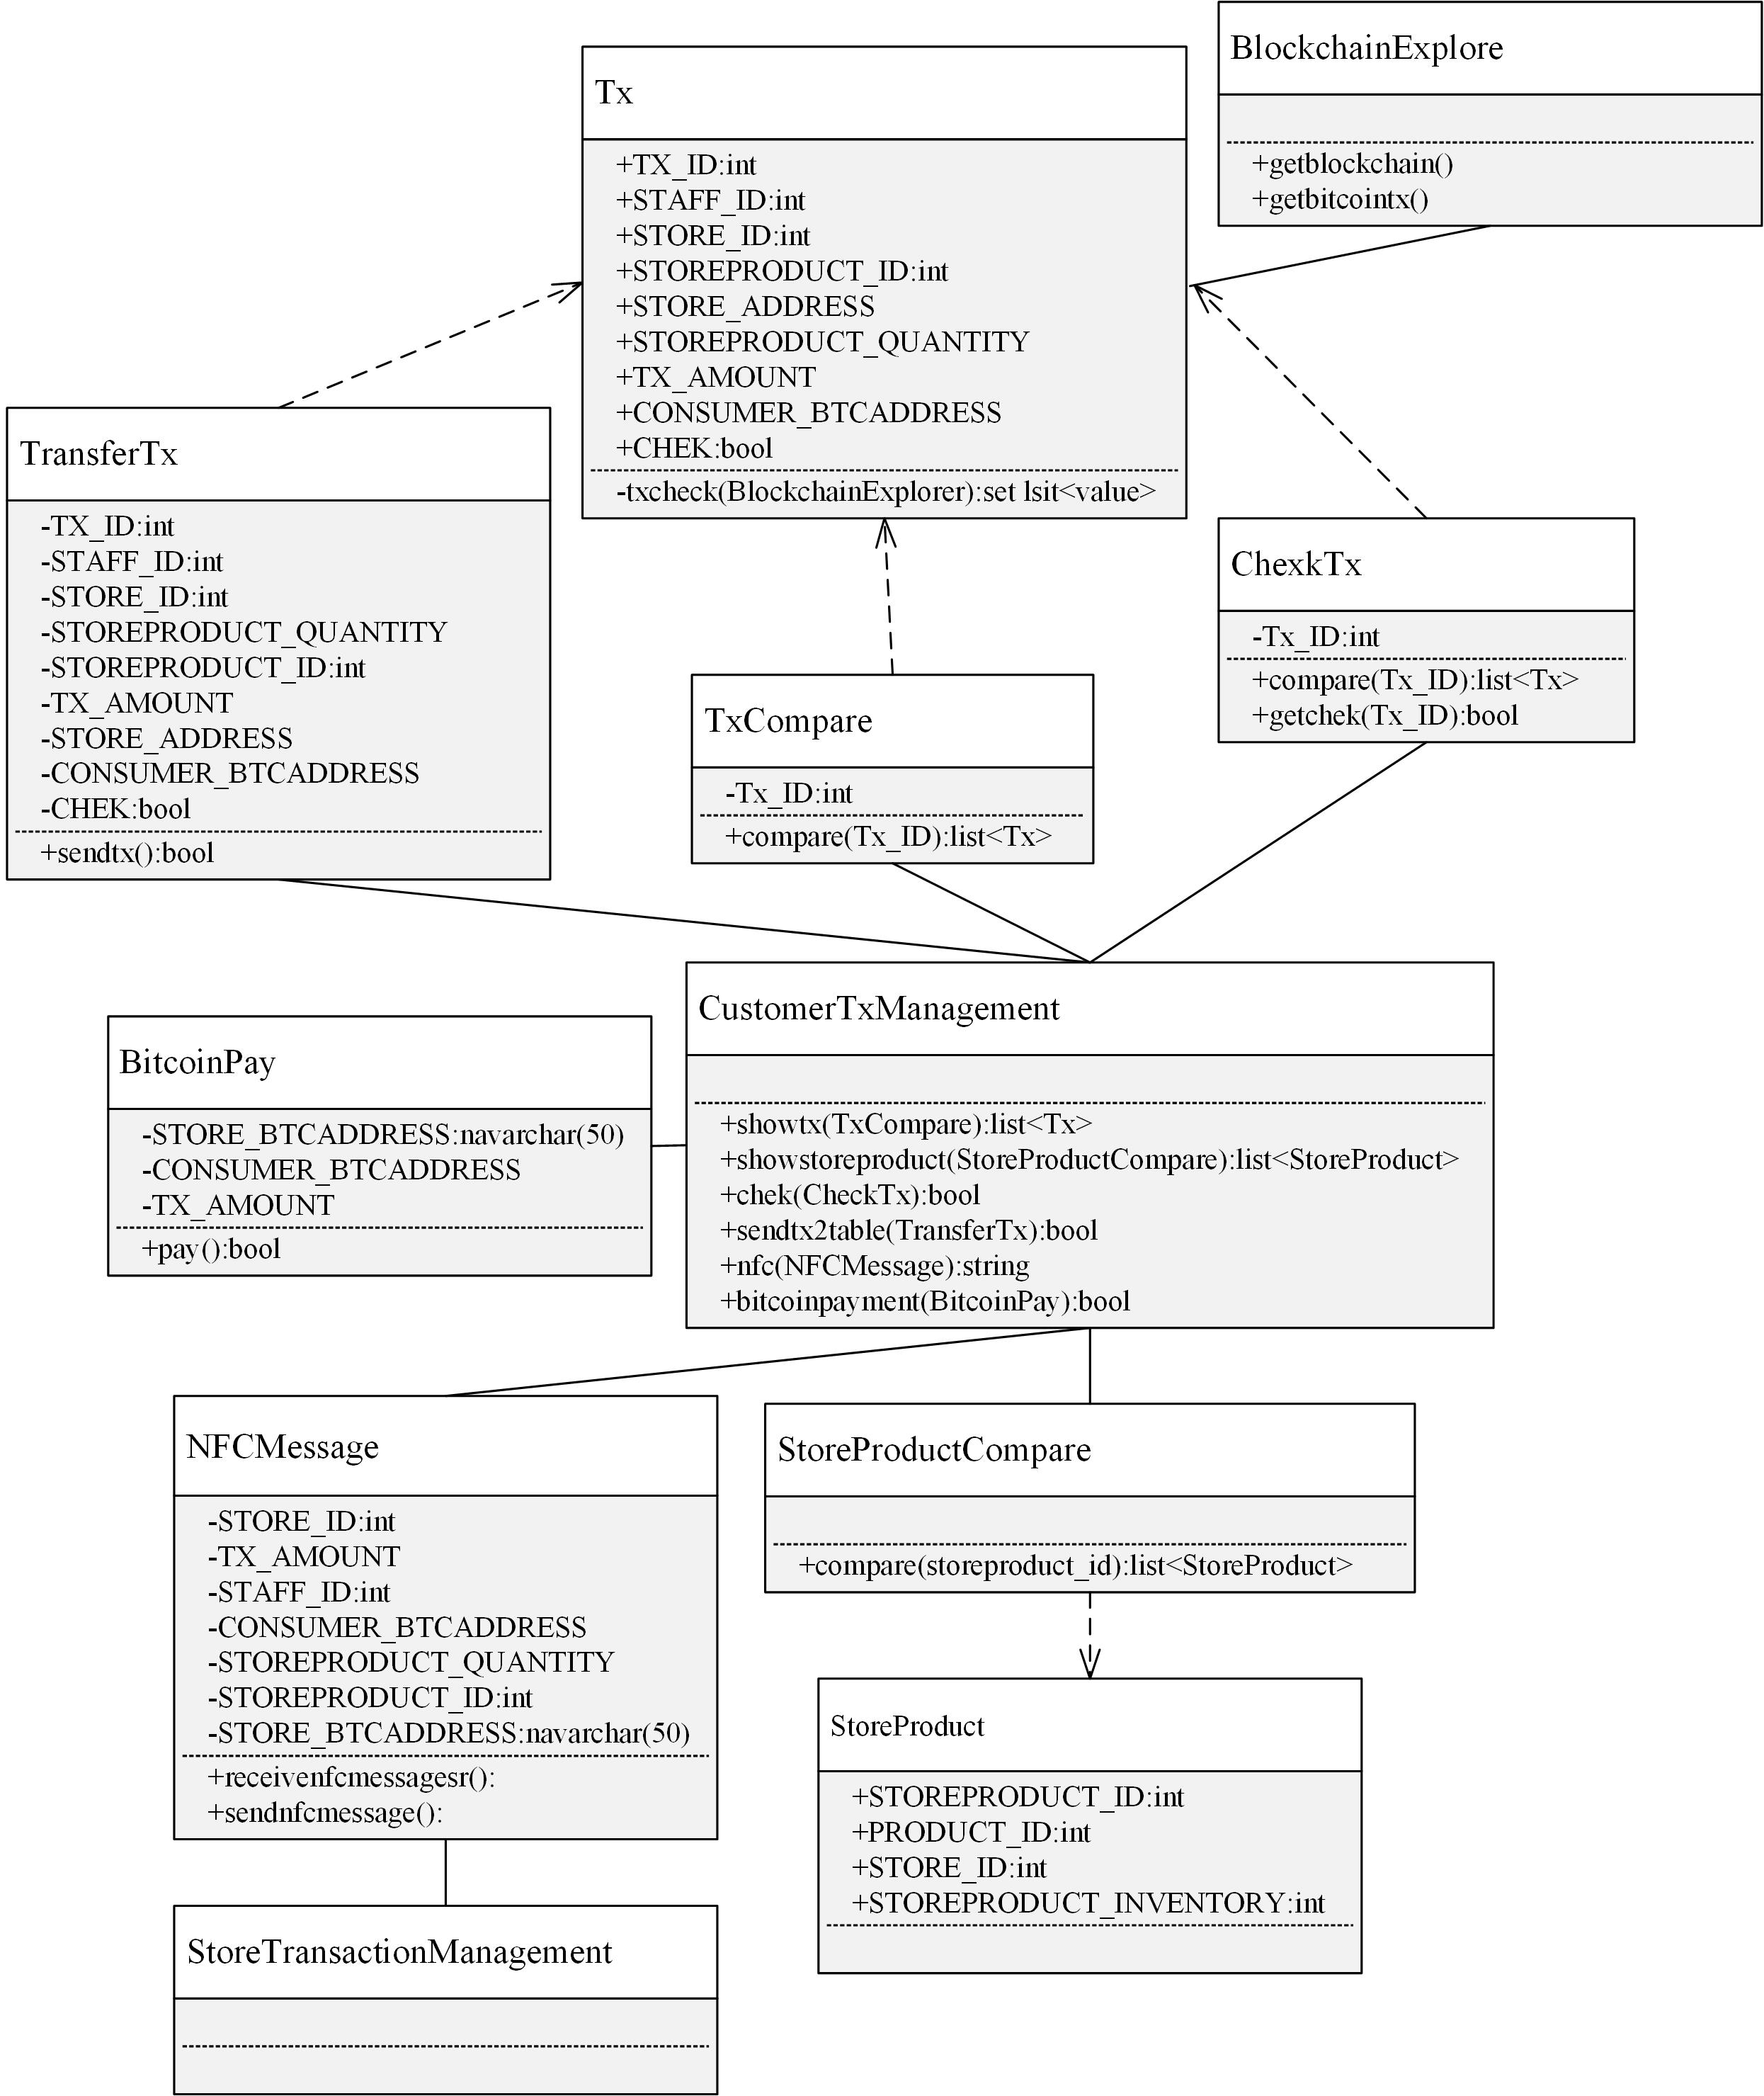
\includegraphics[width = 0.9\textwidth]{c4.pdf}
		\caption{顾客交易管理模块类图}\label{c4}
	\end{figure}

	

	图\ref{time5}为顾客交易管理时序图,以下为流程说明:

	\begin{figure}[!htbp]
		\centering
		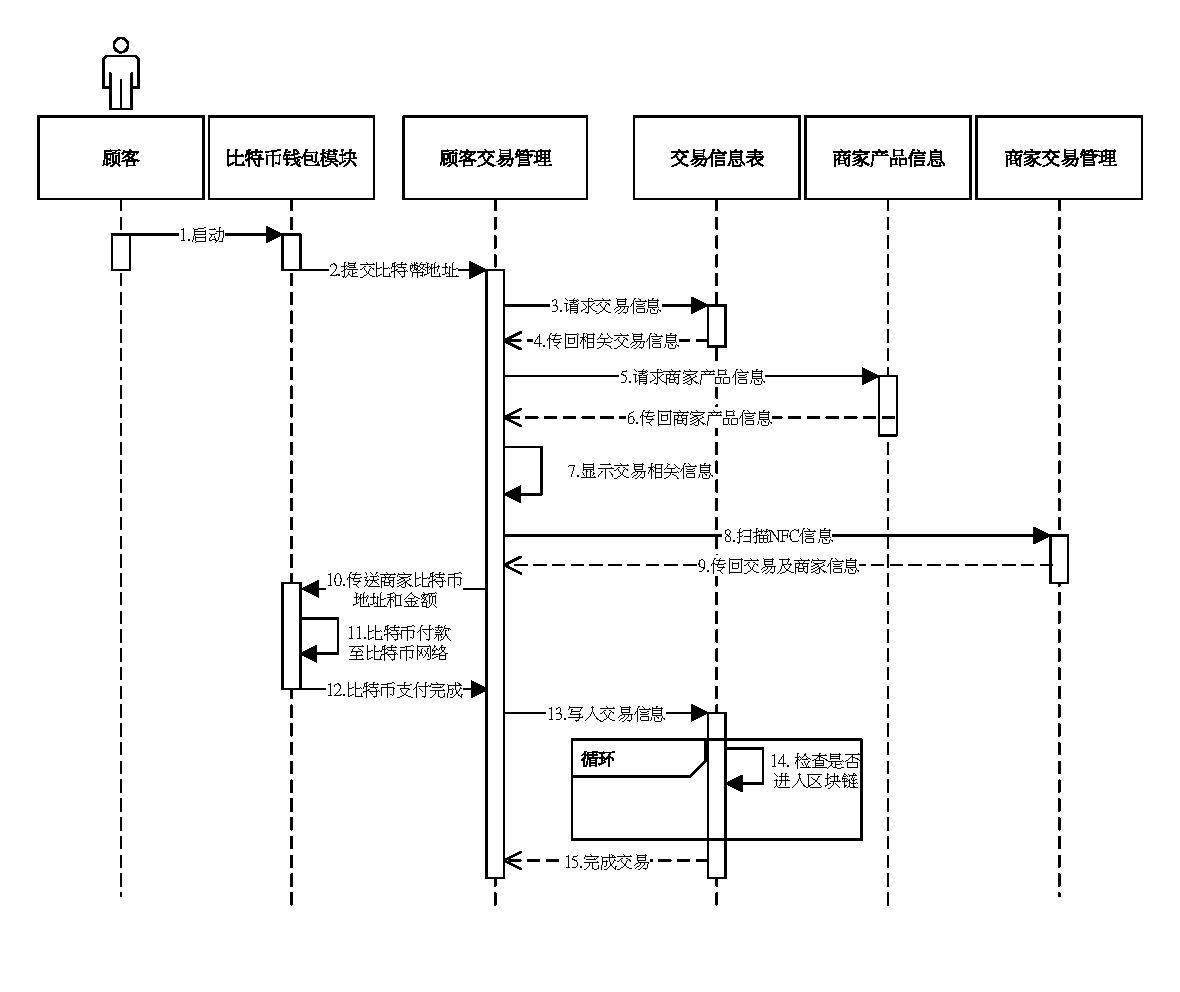
\includegraphics[width = 1\textwidth]{time5.pdf}
		\caption{顾客交易管理时序图}\label{time5}
	\end{figure}

	\begin{enumerate}
		\item 顾客启动比特币钱包管理模块,届时比特币钱包管理模块再同步最新的区块链信息至手持移动装置,并将与手持移动装置本身存在的比特币地址进行核对。
		\item 将所有在比特币钱包模块的地址提交到顾客交易管理模块。
		\item 顾客交易管理模块将所有拿到的比特币地址发送到交易信息表,请求完整的交易信息内容。
		\item 交易信息表将概要的交易信息传回顾客交易管理,此时的交易信息并非相当完整,只有商家产品编号。
		\item 为了使得交易信息更加的完整可以显示更多的商家产品说明,便将手持移动装置数据库存在的商家产品编号向商家产品信息表提出请求更详细的说明。
		\item 商家产品信息表传回详细的商家产品信息到顾客交易管理模块。
		\item 顾客交易管理模块将收到的信息显示在画面上。
		\item 当顾客前往商家时,商家扫描完所有顾客欲购买的商家比特币地址、商家商品、数量、价格以及应付金额之后,便向商家交易管理启动NFC准备等待顾客的手持设备进行信息传输,此时的顾客将手持设备与商家手持设备靠近。
		\item 商家管理模块透过NFC将交易清单信息发送到顾客交易管理模块。
		\item 在商家交易管理模块重送的交易清单信息当中,包括商家的比特币地址信息与应付金额,此时顾客交易管理模块将比特币地址信息发送到比特币钱包模块。
		\item 在比特币钱包模块当中使用secp256k1算法签署比特币交易信息,并将交易信息广播到比特币网络当中,此时该笔交易信息会进到⽐特币网络中的交易缓存池等待矿工解出工作量证明的问题,将该笔交易信息存储到比特币区块链。
		\item 在完成比特币签名后,会生成比特币的交易哈希值,比特币钱包管理模块将比特币交易哈希值发送到顾客交易管理模块。
		\item 顾客交易管理模块请求交易信息表将比特币交易哈希值写入。
		\item 完成写入后,交易信息表模块会调用比特币区块链检视器的相关函数,不断检查该笔比特币交易是否已经从未确认交易转变成已确认交易。倘若发现已经确认,则将交易信息表中CHECK字段的信息从"0"修改为"1"。
		\item 发现交易信息中的CHECK值为"1"之后,便发送完成交易的信息到顾客交易管理模块。
	\end{enumerate}

	图\ref{c6}为BRTMS中的顾客Government Green Address交易管理模块类图,以下将说明采用Government Green Address与未采用Government Green Address技术的顾客交易管理类图设计之间的差异。于Tx类中添加ggatxcheck()方法,该方法可以不断检查交易信息表中的交易是否来自Government Green Address地址,倘若是则不需要等待区块链的验证时间可以即刻认定该笔交易为有效,快速提交比特币交易速度。GovernmentGreenaddressCheckTx类中compare()方法是为了查找与TX\_ID相符的交易信息,getchek()方法则是向交易信息表中询问符合TX\_ID的交易信息是否已经被修改为"1"。其中GovernmentGreenaddressBitcoinPay类中的multiplesignature()方法可以实现多重签章算法,使得本系统可以支持即时交易。governmentgreedaddresspay()方法是将多重签章算法广播报导比特币网络。


	\begin{figure}[!htbp]
		\centering
		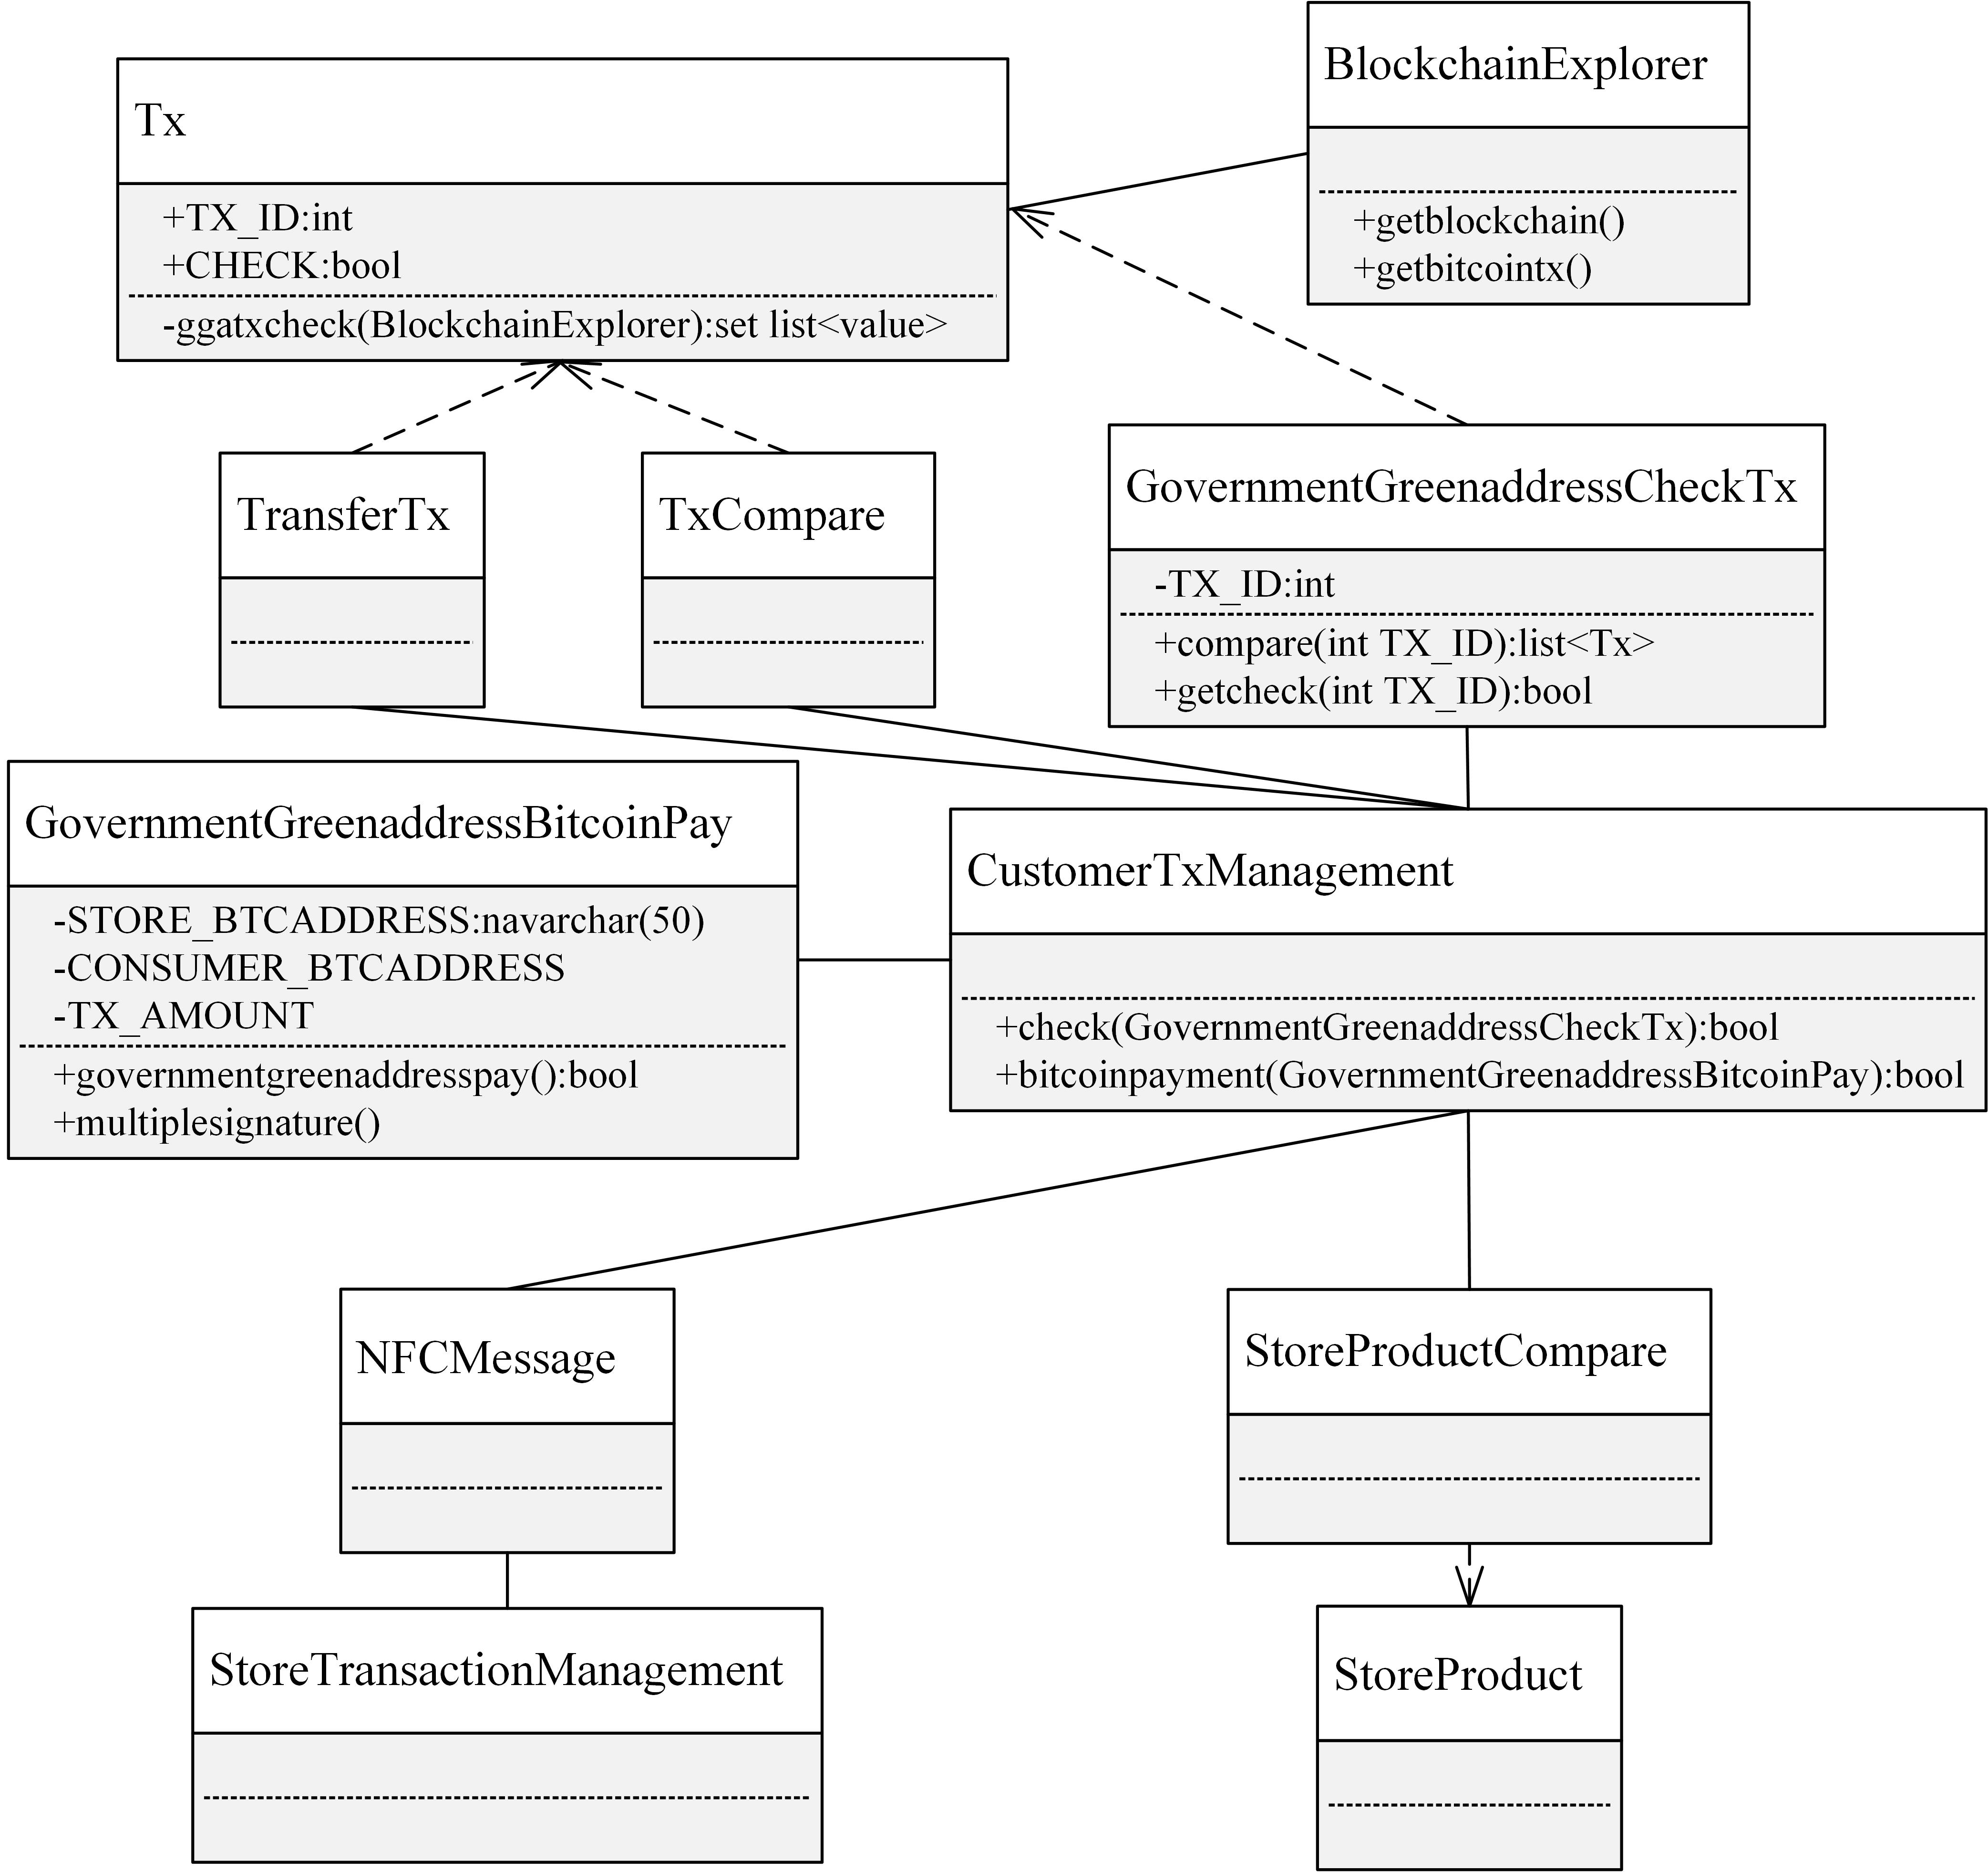
\includegraphics[width = 0.7\textwidth]{c6.pdf}
		\caption{顾客Government Green Address交易管理模块类图}\label{c6}
	\end{figure}

\section{系统实现}

% \section{区块链的实名交易监督系统实现}

为了验证和证明所提议的BTMS用于比特币支付收款监督的可行性和有效性,将其运行在用于商家商品管理和维护的Java应用程序的SMIMSS子系统,用于商家职工的运行在手持移动装置上的SMCTSS子系统以及运行在顾客手持移动装置上的CMPTSS子系统。
如图\ref{fig5}所示,SMIMSS 的 Java应用程序可以帮助商家登入到系统或创建一个新帐户。 授权商家成功登⼊系统后,商家可以插⼊或更新产品列表,实现的SMIMSS Java 应⽤程序运⾏前⾯部分中所述的功能,如图\ref{fig6}所示。

\begin{figure}[!htbp]
	\centering
	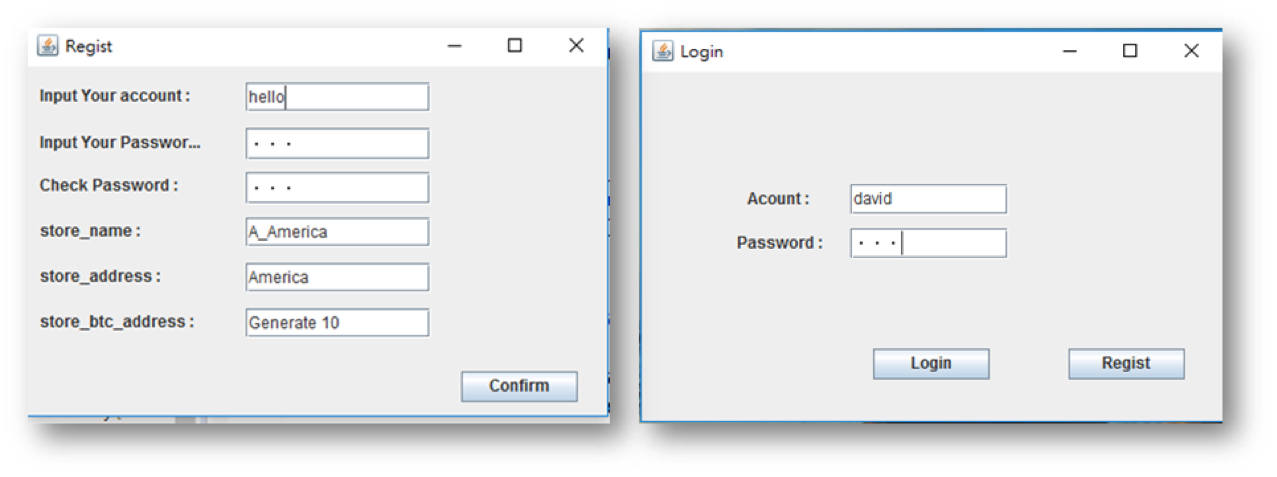
\includegraphics[width = 0.9\textwidth]{fig5.png}
	\caption{SMIMSS的Java应用程序的注册和登入界面}\label{fig5}
\end{figure}

\begin{figure}[!htbp]
	\centering
	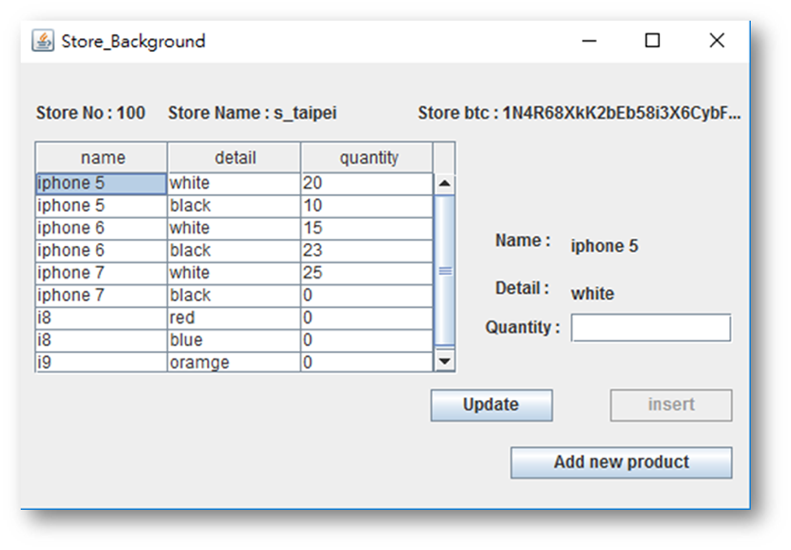
\includegraphics[width = 0.6\textwidth]{fig6.png}
	\caption{在SMIMSS中插入或更新授权商家的产品目录}\label{fig6}
\end{figure}

商家的产品信息可以通过RFID标签扫描,存储到云端数据库中,商家职工可以使用实现的SMCTSS 手持移动装置App 客户端,启用NFC监听器,从购物车中的顾客购买产品中读取RFID标签信息。 在如图\ref{fig7}所示的第一项活动中,商家职工必须登入才能获得授权访问SMCTSS子系统功能。 然后,在第二项活动中,SMCTSS应用程序可以通过使用SMIMSS子系统中应用的云数据库检查产品RFID标签信息并将其展示给顾客,从而将扫描的产品列入购物车。 在图\ref{fig7}的第三项活动中,顾客可以要求职工删除购买物品以,并确认最终交易清单。 最后,SMCTSS应用程序将自动使用比特币测试网络(Bitcoin Testnet)\supercite{bitcointestnet}帮助职工确认发布此比特币交易的收款人地址,如图\ref{fig7}的最后一个步骤所示。    

\begin{figure}[!htbp]
	\centering
	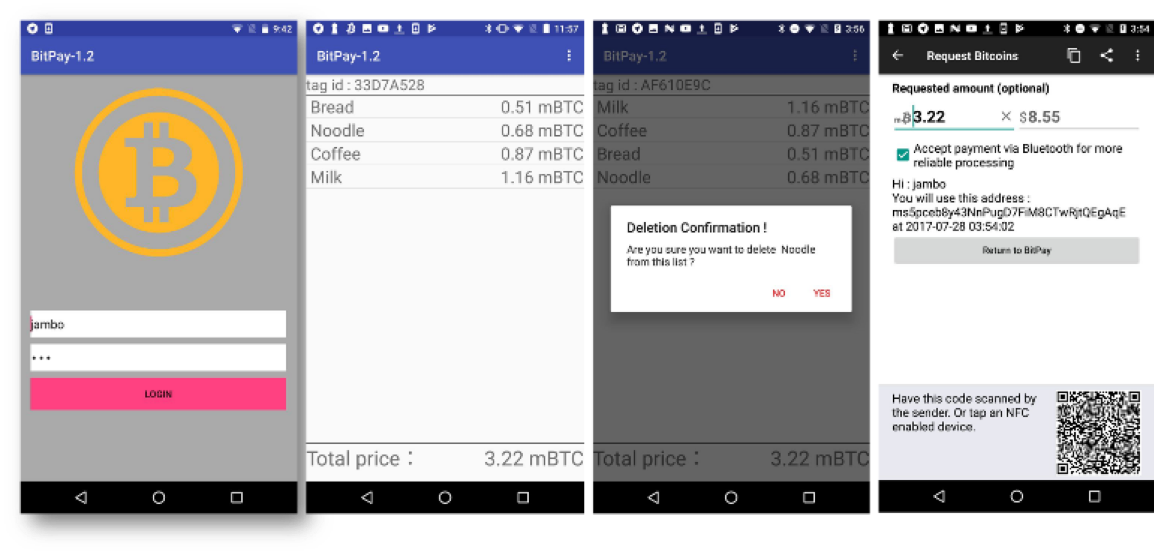
\includegraphics[width = 1\textwidth]{fig7.png}
	\caption{登入、等待结帐的商品、删除商品及支付确认}\label{fig7}
\end{figure}

同时,顾客将使用与SMCTSS 子系统客户端相对应的CMPTSS 子系统客户端通过比特币完成采购产品交易。 如图\ref{fig8}所示,第一个活动表示顾客确认购买产品创建交易数据库的交易清单,第二个活动显示包括金额和付款人比特币地址在内的付款确认,第三个活动显⽰该钱包交易的历史记录,凡是出入该钱包的所有交易都会被显示出来,
钱包可以同时作为买⽅和卖⽅,最后在第四项活动中显示了该笔交易详细采购产品的交易凭据。    

\begin{figure}[!htbp]
	\centering
	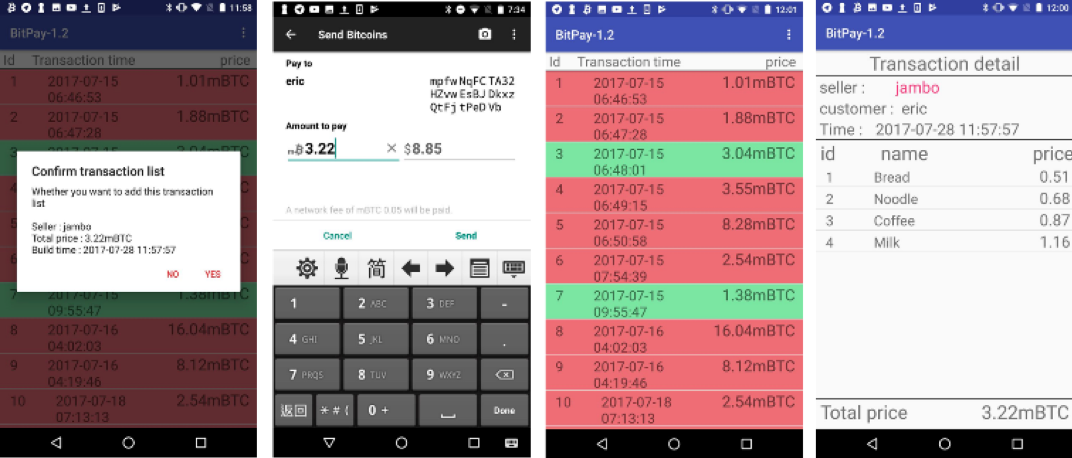
\includegraphics[width = 1\textwidth]{fig8.png}
	\caption{在CMPTSS App中,交易确认,付款确认、交易历史记录和交易凭证}\label{fig8}
\end{figure}